En el presente capítulo se explica la experimentación 
realizada para la clasificación de los videos del 
\textit{dataset Hockey Fights}. La 
estructura que se detalla a continuación consiste de: 
explicación del \textit{pipeline}, la experimentación 
con las diferentes configuraciones de BI-LSTM y la 
comparativa de los resultados.

\section{Pipeline propuesto}

La Imagen \ref{metodologia} ilustra la metodología propuesta, 
la cual se procederá a explicar a continuación:

\begin{figure}[h!] 
    \includegraphics[width=0.7\textwidth]{images/metodologiaMaestria.png} 
    \centering 
    \caption{Metodología propuesta. Creación propia.} 
    \label{metodologia} 
\end{figure}

El \textit{pipeline} consiste en la obtencion, preprocesamiento 
y almacenamiento de las caracteristicas obtenidas del 
\textit{dataset}, para luego ser pasado a las diferentes 
configuraciones de los modelos BI-LSTM, los cuales se 
encargarán cada video basado en sus frames y finalmente 
se evaluarán los resultados basados en la métrica f1 y 
el tiempo de inferencia.

\subsection{Extracción de frames y preprocesamiento}

Como primer paso de la metodología se necesitó realizar un 
preprocesamiento de los datos para su análisis posterior a 
través de los modelos mencionados en el anterior capítulo. 
Como primer paso, se procedió a descargar el 
\textit{dataset} a través de su repositorio de 
\href{https://www.kaggle.com/datasets/yassershrief/hockey-fight-vidoes/data}{Kaggle}. \\

Una vez obtenidos los datos, se procedió a etiquetar cada uno 
de los videos basados en los nombres de cada uno de ellos. 
Se puede diferenciar su etiqueta debido a que aquellos que 
comiencen con "fi" contienen violencia, mientra que los demás, 
no. Con los videos cargados, se recolectaron los frames tal 
como fue mencionado anteriormente. Para ello, se decidió 
hacer un muestreo de 10 frames de manera equitativamente 
separada del video (1 por cada 4 frames). Cada uno de estos 
frames fueron redimensionados a un formato estandar (224 x 224) 
para luego ser normalizados.

\subsection{Obtención de las características}

Con cada conjunto de frames por video, estos pasan a través de 
las diferentes arquitecturas de CNN mencionadas en el anterior 
capítulo. Para ello, se tuvieron las siguientes consideraciones: 
\begin{itemize}
    \item Se obtendrán los modelos pre-entrenados con el 
    dataset ImageNet.
    \item Se eliminan las capas de clasificación.
    \item Se agrega una capa GlobalAveragePooling2D para 
    reducir la dimensionalidad de kernels(resultado de las CNN). 
    \item Se marca al modelo final como no entrenable.
\end{itemize}
 
Este ultimo paso es necesario debido a que se utilizará el 
conocimiento pre-entrenado de los modelos para obtener 
únicamente el vector característico de cada una de las 
imágenes. En ese sentido, se hace innecesario el proceso de 
entrenamiento de estas. Además, sería contraproducente tanto 
entrenar una CNN basado únicamente en frames porque pueden 
existir casos en el que existen frames donde no hay violencia 
y viceversa y también debido a que se perdería parte del 
conocimiento que ya tienen estos modelos. Finalemente se 
procedió a guardar estos vectores de características en 
formato h5. \\

Cabe resaltar que en la realidad podría implementarse un 
modelo conjunto con la CNN y LSTM, pero algunos de los modelos 
(especialmente los EfficientNet) contienen capas que no son 
facilmente mapeables a las entradas de las BI-LSTM, por lo 
cual se tuvo que hacer esto como  preprocesamiento.

\subsection{Entrenamiento y prueba del clasificador}

Como clasificador, se tuvo un modelo de BI-LSTM con diferente 
número de celdas. Para esta experimentación, se decidió usar 
un número entre 1 y 9 celdas, ya que consistía en un dataset 
bastante sencillo y altamente estudiado anteriormente. 

Para cada uno de las CNN's mencionadas en la anterior sección, 
y para cada una de las configuraciones, se procedió a 
entrenar y testear cada combinación de ellas. Las consideraciones 
para esta arquitectura fueron las siguientes:

\begin{itemize}
    \item De entrada se tienen los vectores de características 
    obtenidos del paso anterior (se debe considerar que los 
    tamaños de salida puden variar con respecto a la CNN). 
    \item Se crea un modelo BI-LSTM con X celdas, 10 timesteps 
    (en otras palabras los 10 frames obtenidos) y el tamaño 
    del output del anterior paso.
    \item Capas densas de 1024, 50 y 2 neuronas con funciones 
    de activación RelU y la última de tipo softmax. 
    \item Función de pérdida Binary CrossEntropy, optimizador adam 
    y de métricas accuracy y f1-score.
    \item Función de early stopping con \textit{patience} de 3 y  
    \textit{min delta} de 0.005 y batch de 16 videos por vez.
\end{itemize}

En la siguiente sección se presentarán los resultados 
generados utilizando las anteriores consideraciones para 
cada uno de los modelos mencionados.

\section{Experimentación}

Como primer paso, se procedió a realizar el pre-procesamiento 
de las imágenes y la obtención de sus características tal 
como fue mencionado anteriormente. Para ello, se recolectaron 
las métricas acerca de la cantidad de parámetros y el 
tiempo de cálculo de cada uno de los modelos, los cuales 
se puden observar en la Tabla \ref{tabla:procesamiento}:

\begin{table}[h!]
\centering
\begin{tabular}{|l|r|r|}
\hline
\multicolumn{1}{|c|}{\textbf{Modelo}} & \multicolumn{1}{c|}{\textbf{Parámetros}} & \multicolumn{1}{c|}{\textbf{\begin{tabular}[c]{@{}c@{}}Timpo de inferencia\\ (por batch de 10)\\ en ms/batch\end{tabular}}} \\ \hline
\textbf{efficientnetb0}               & 4,049,571                                & 46 ms                                                                                                                       \\ \hline
\textbf{resnet50}                     & 23,587,712                               & 51 ms                                                                                                                       \\ \hline
\textbf{efficientnetv2-s}             & 20,331,360                               & 75 ms                                                                                                                       \\ \hline
\textbf{MobilenetV3large}             & 2,996,352                                & 45 ms                                                                                                                       \\ \hline
\end{tabular}
\label{tabla:preprocesamiento}
\end{table}

Se puede apreciar que el tamaño final de los modelos fue 
menor que el esperado por la Tabla \ref{evaluacion}. 
Esto se debió a que no se están utilizando las capas densas 
de los modelos y se estan reemplazando con una capa 
GlobalAveragePooling2D, la cual obtiene el resultado del 
kernel final de las capas convolucioanles y las reduce a un 
solo resultado promediado. 

Habiendo obtenido las características de cada uno de las 
imágenes y los diez frames generados por cada uno de ellas, 
se entrenaron diferentes modelos BI-LSTM como fue mencionado 
anteriormente, teniendo desde 1 a 10 celdas para cada uno de 
los CNN utilizados. A continuación se muestran las gráficas 
de pérdida y f1 score para cada una de los experimentos. 

\begin{figure}[h!]
    \centering
    \subfloat[\centering F1 score por época]{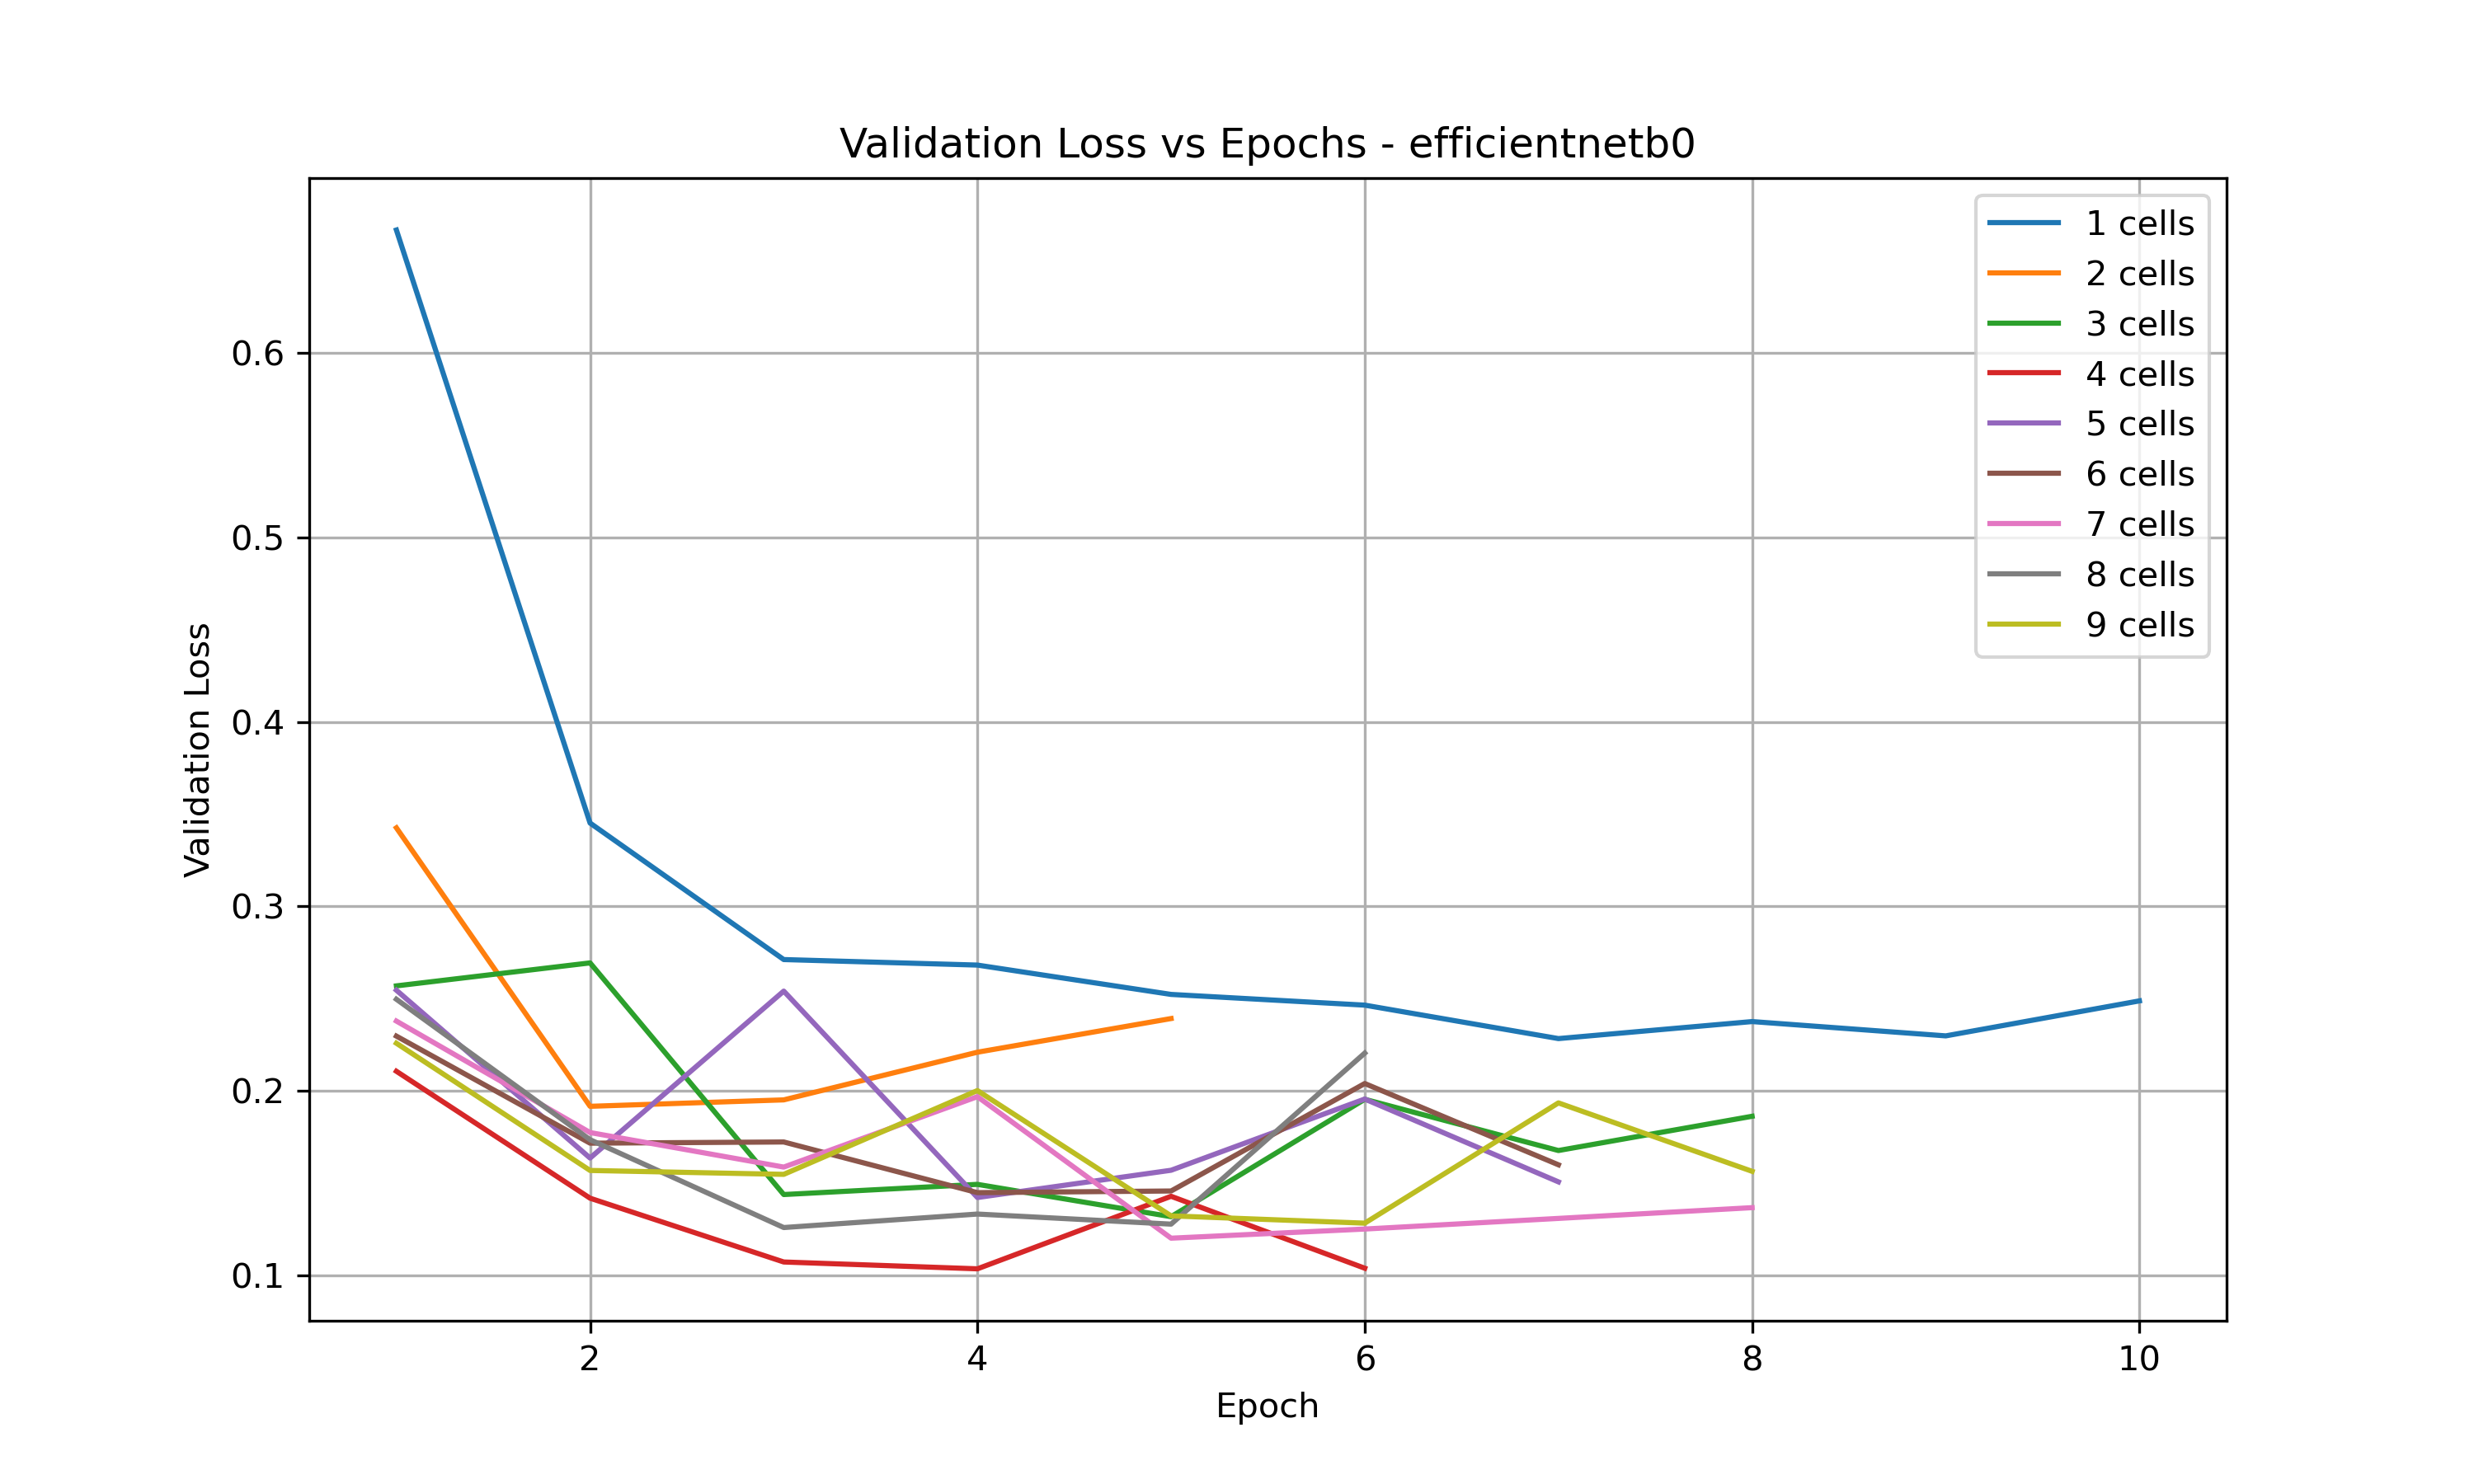
\includegraphics[width=0.48\textwidth]{../graphs/efficientnetb0_val_loss_per_epoch.png}}
    \subfloat[\centering Pérdida por época]{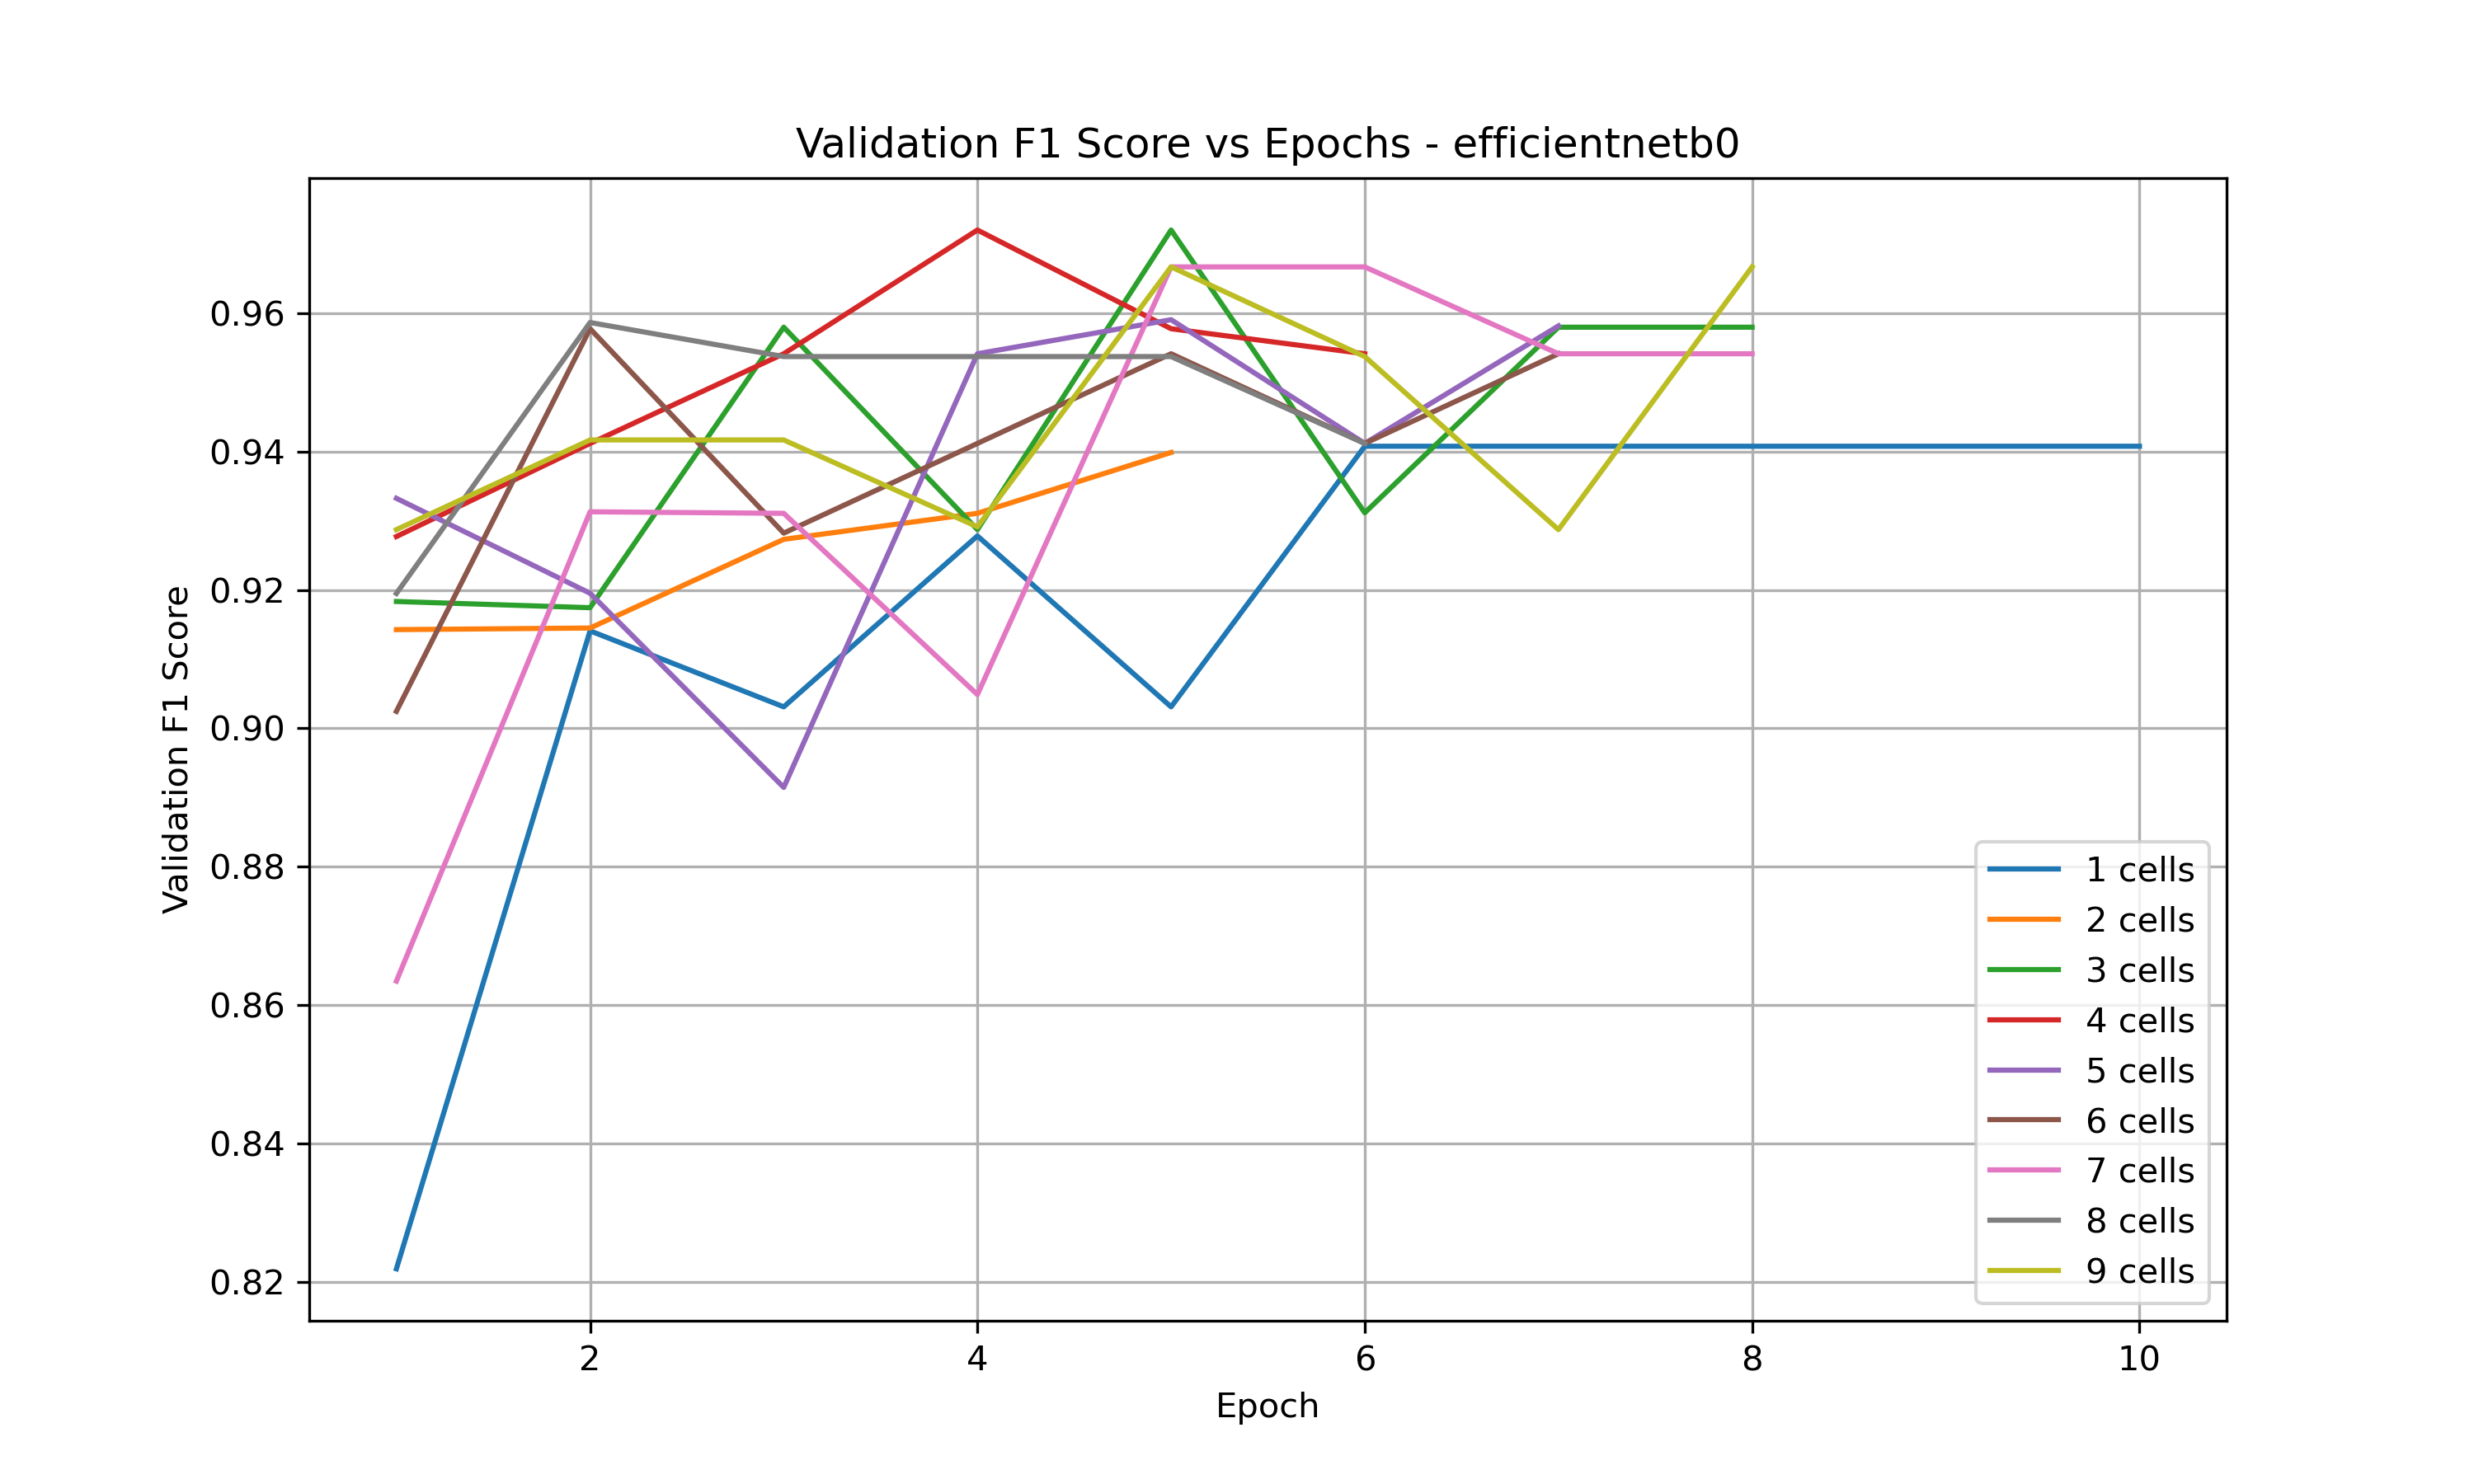
\includegraphics[width=0.48\textwidth]{../graphs/efficientnetb0_val_f1_per_epoch.png}}\hfill
    \caption{Gráficos de pérdida y f1 score por época usando EfficientNetB0}
    \label{fig:combinedEfficientnetB0}
\end{figure}

Los gráficos de la figura \ref{fig:combinedEfficientnetB0} muestran 
un descenso de la pérdida generada de manera estable, en donde el 
clasificador con 1 capa se puede apreciar muy separado de las demás 
configuraciones. Fuera de ella, todas las demás configuraciones obtuvieron 
resultados muy similares. Sin embargo, se puede apreciar que la 
configuración con 4 celdas fue la que mejor resultado obtuvo en esa 
métrica. Algo muy similar se ve en la gráfica de f1 score. La configuración 
con una y dos celdas generaron peores resultados, mientras que las demás 
obtuvieron mejores resultados. La diferencia radica en que si consideramos 
el resultado final después de 8 épocas, la configuración con 9 celdas 
es la ganadora. Pero si se considera que el early stopping tenía una paciencia de 
3 épocas, tendríamos que considerar el resultado en la época 6, en donde la 
configuración con 7 celdas fue la que generó mejores resultados. 

\begin{figure}[h!]
    \centering
    \subfloat[\centering F1 score por época]{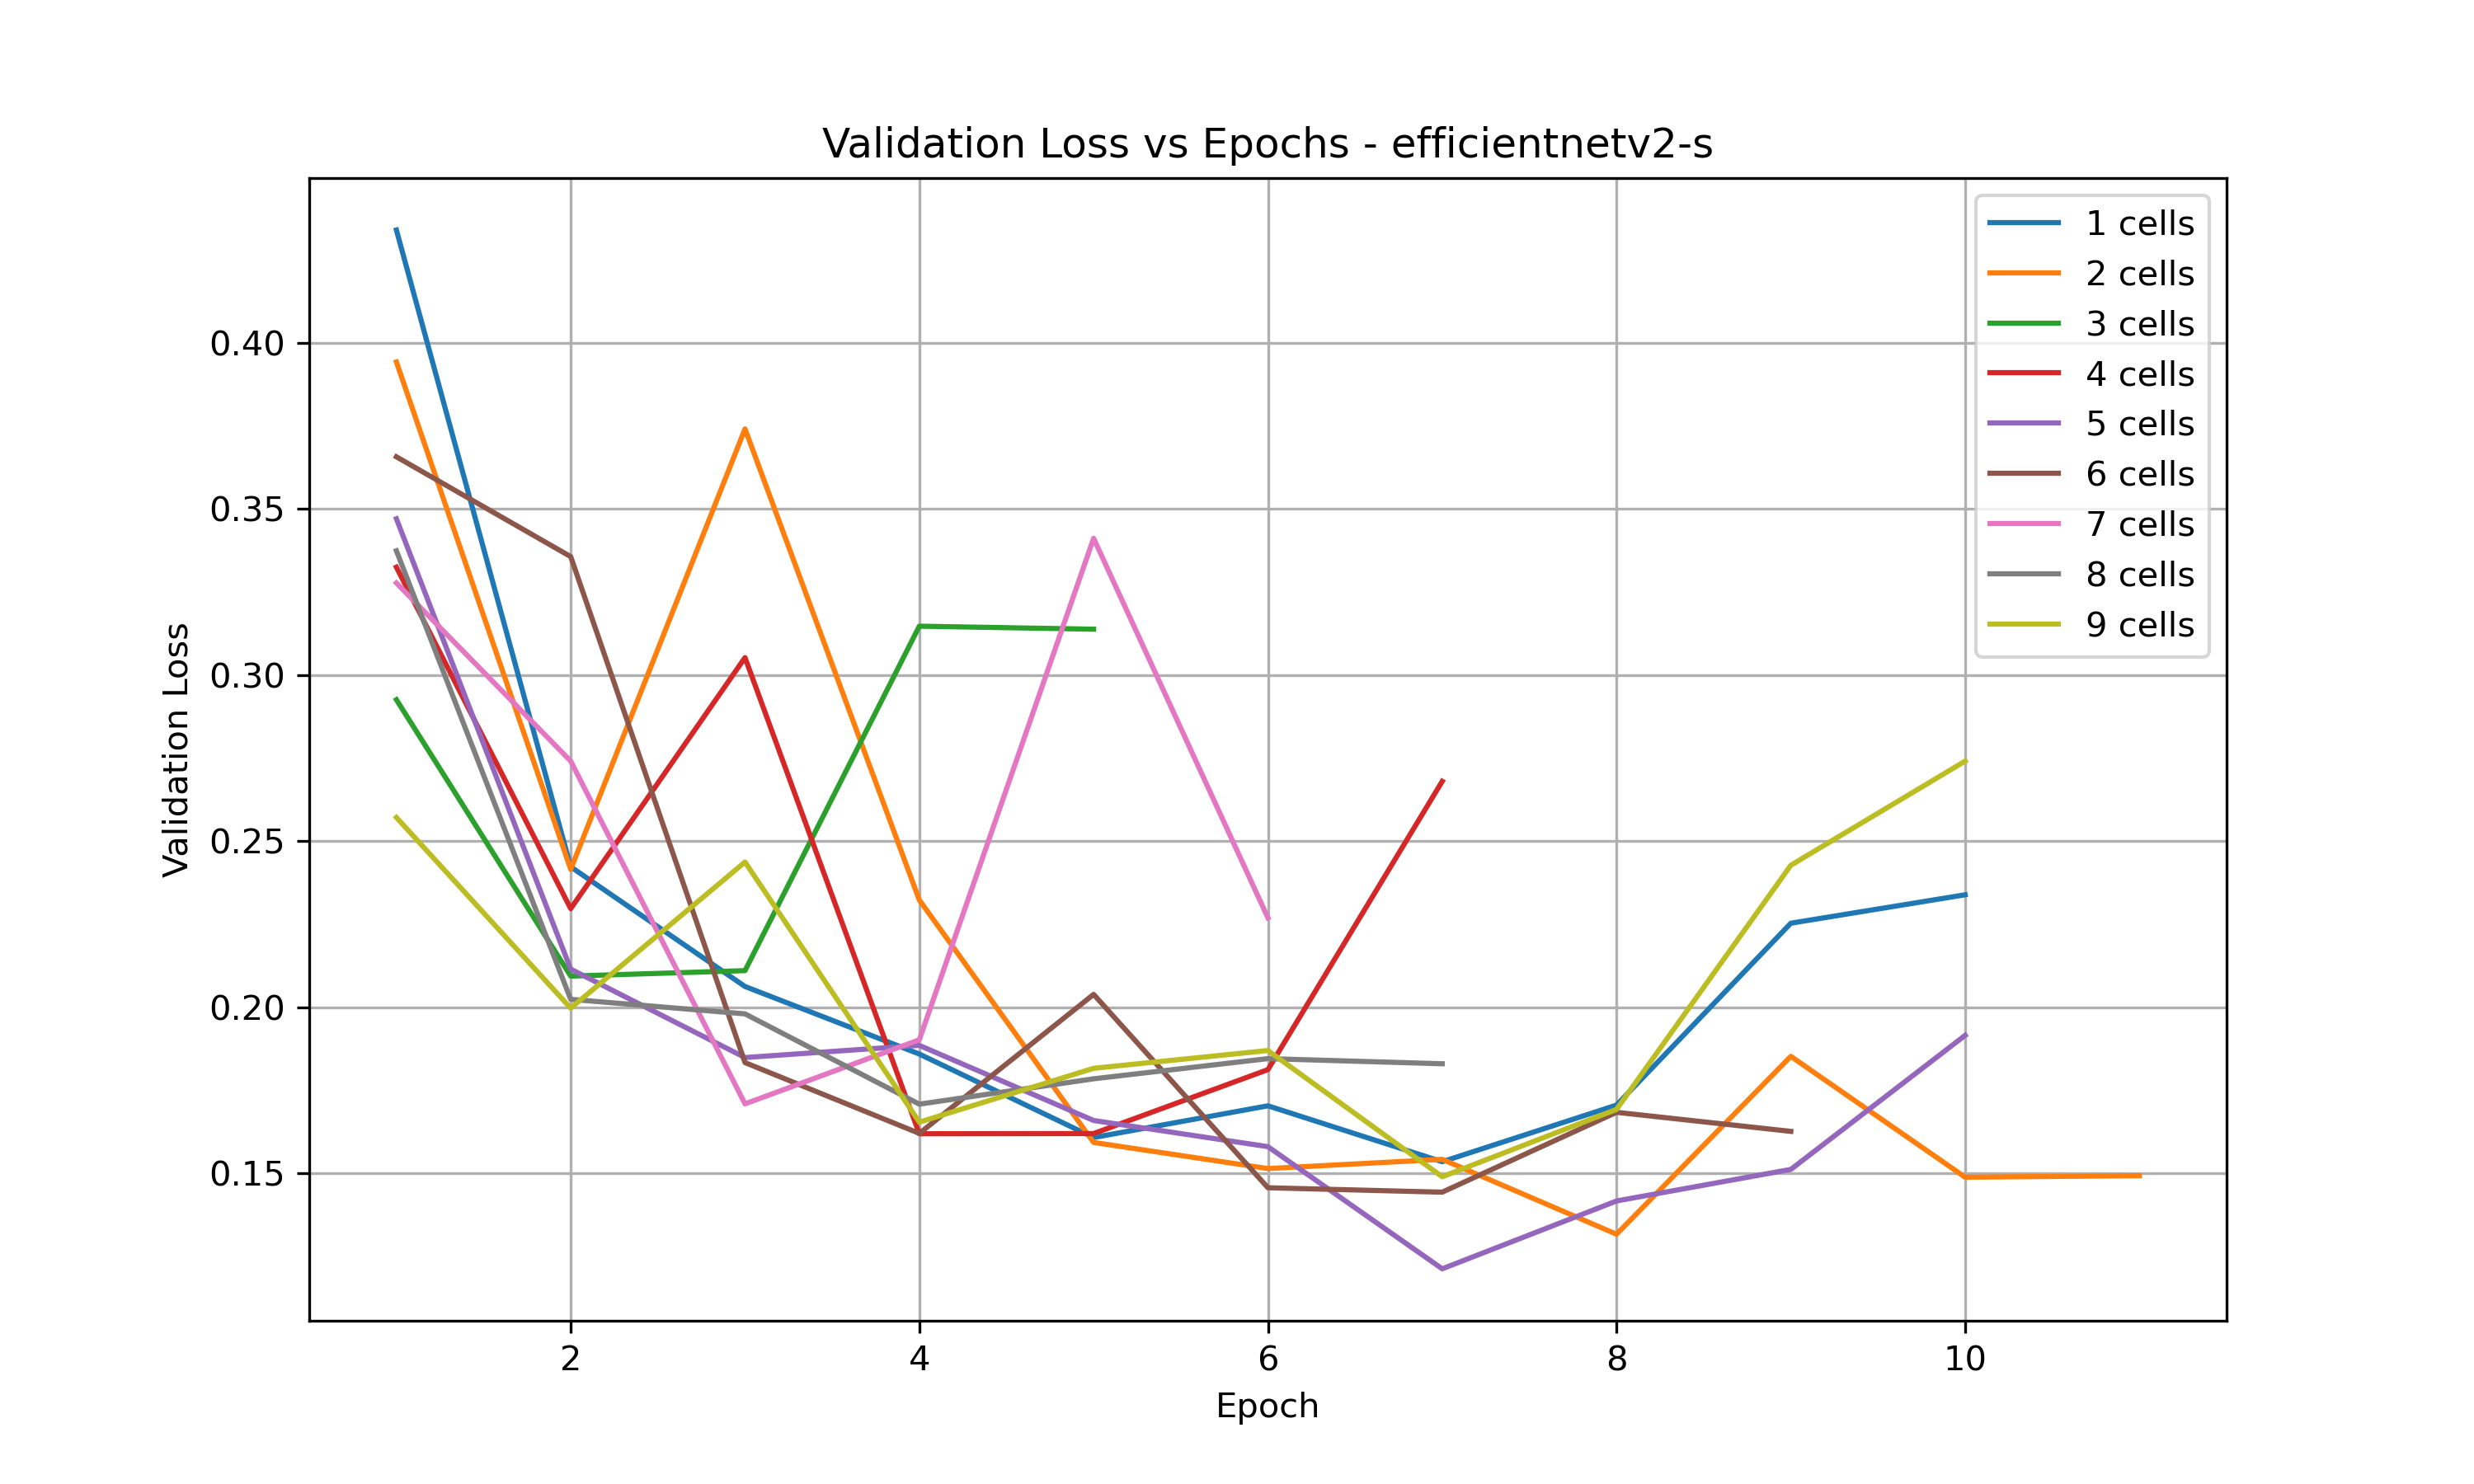
\includegraphics[width=0.48\textwidth]{../graphs/efficientnetv2-s_val_loss_per_epoch.png}}
    \subfloat[\centering Pérdida por época]{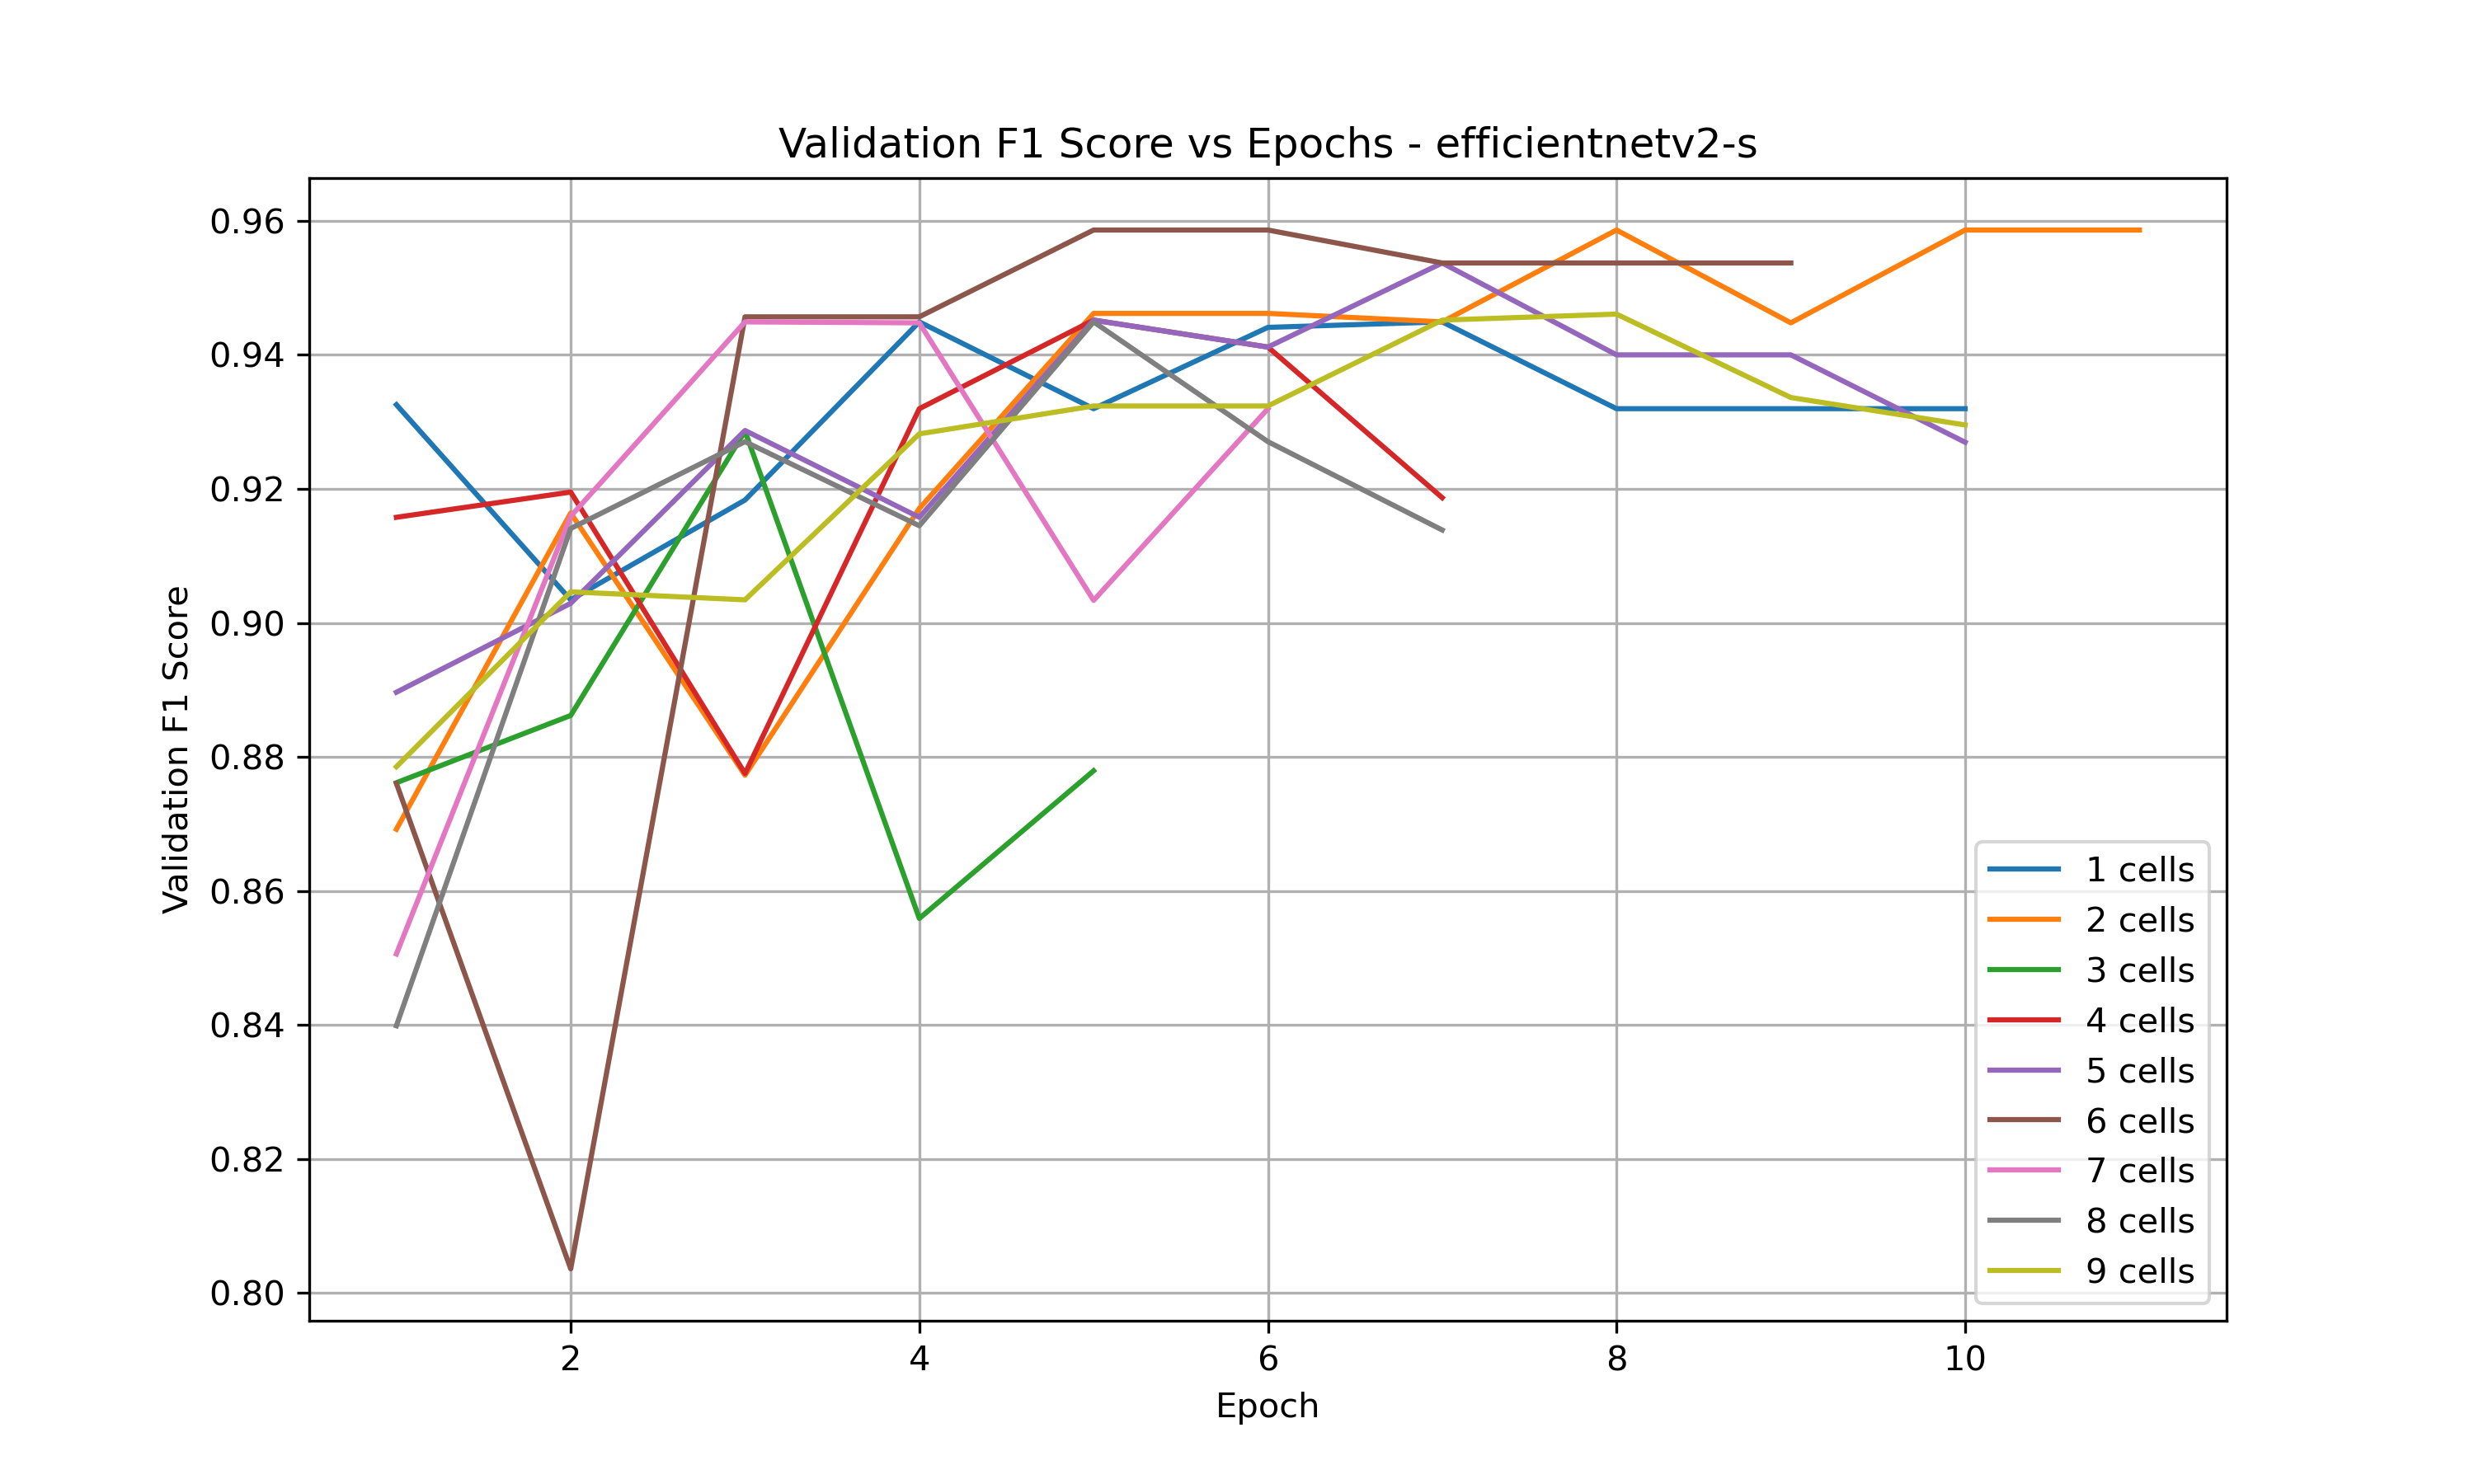
\includegraphics[width=0.48\textwidth]{../graphs/efficientnetv2-s_val_f1_per_epoch.png}}\hfill
    \caption{Gráficos de pérdida y f1 score por época usando EfficinetnetV2-S}
    \label{fig:combinedEfficientnetV2}
\end{figure}

A comparación de la anterior ejecución, los gráficos de la figura 
\ref{fig:combinedEfficientnetV2} muestran un descenso de la pérdida 
gerada menos estable. Los resultados no muestran un patrón único, por 
lo que la única conclusión basada en los datos es que los mejores resultados 
se obtuvieron con 2 y 5 celdas. Por otra parte, en términos de f1 score se 
pudo apreciar un mejor entrenamiento y resultado final en la configuración de 
2 celdas. 

\begin{figure}[h!]
    \centering
    \subfloat[\centering F1 score por época]{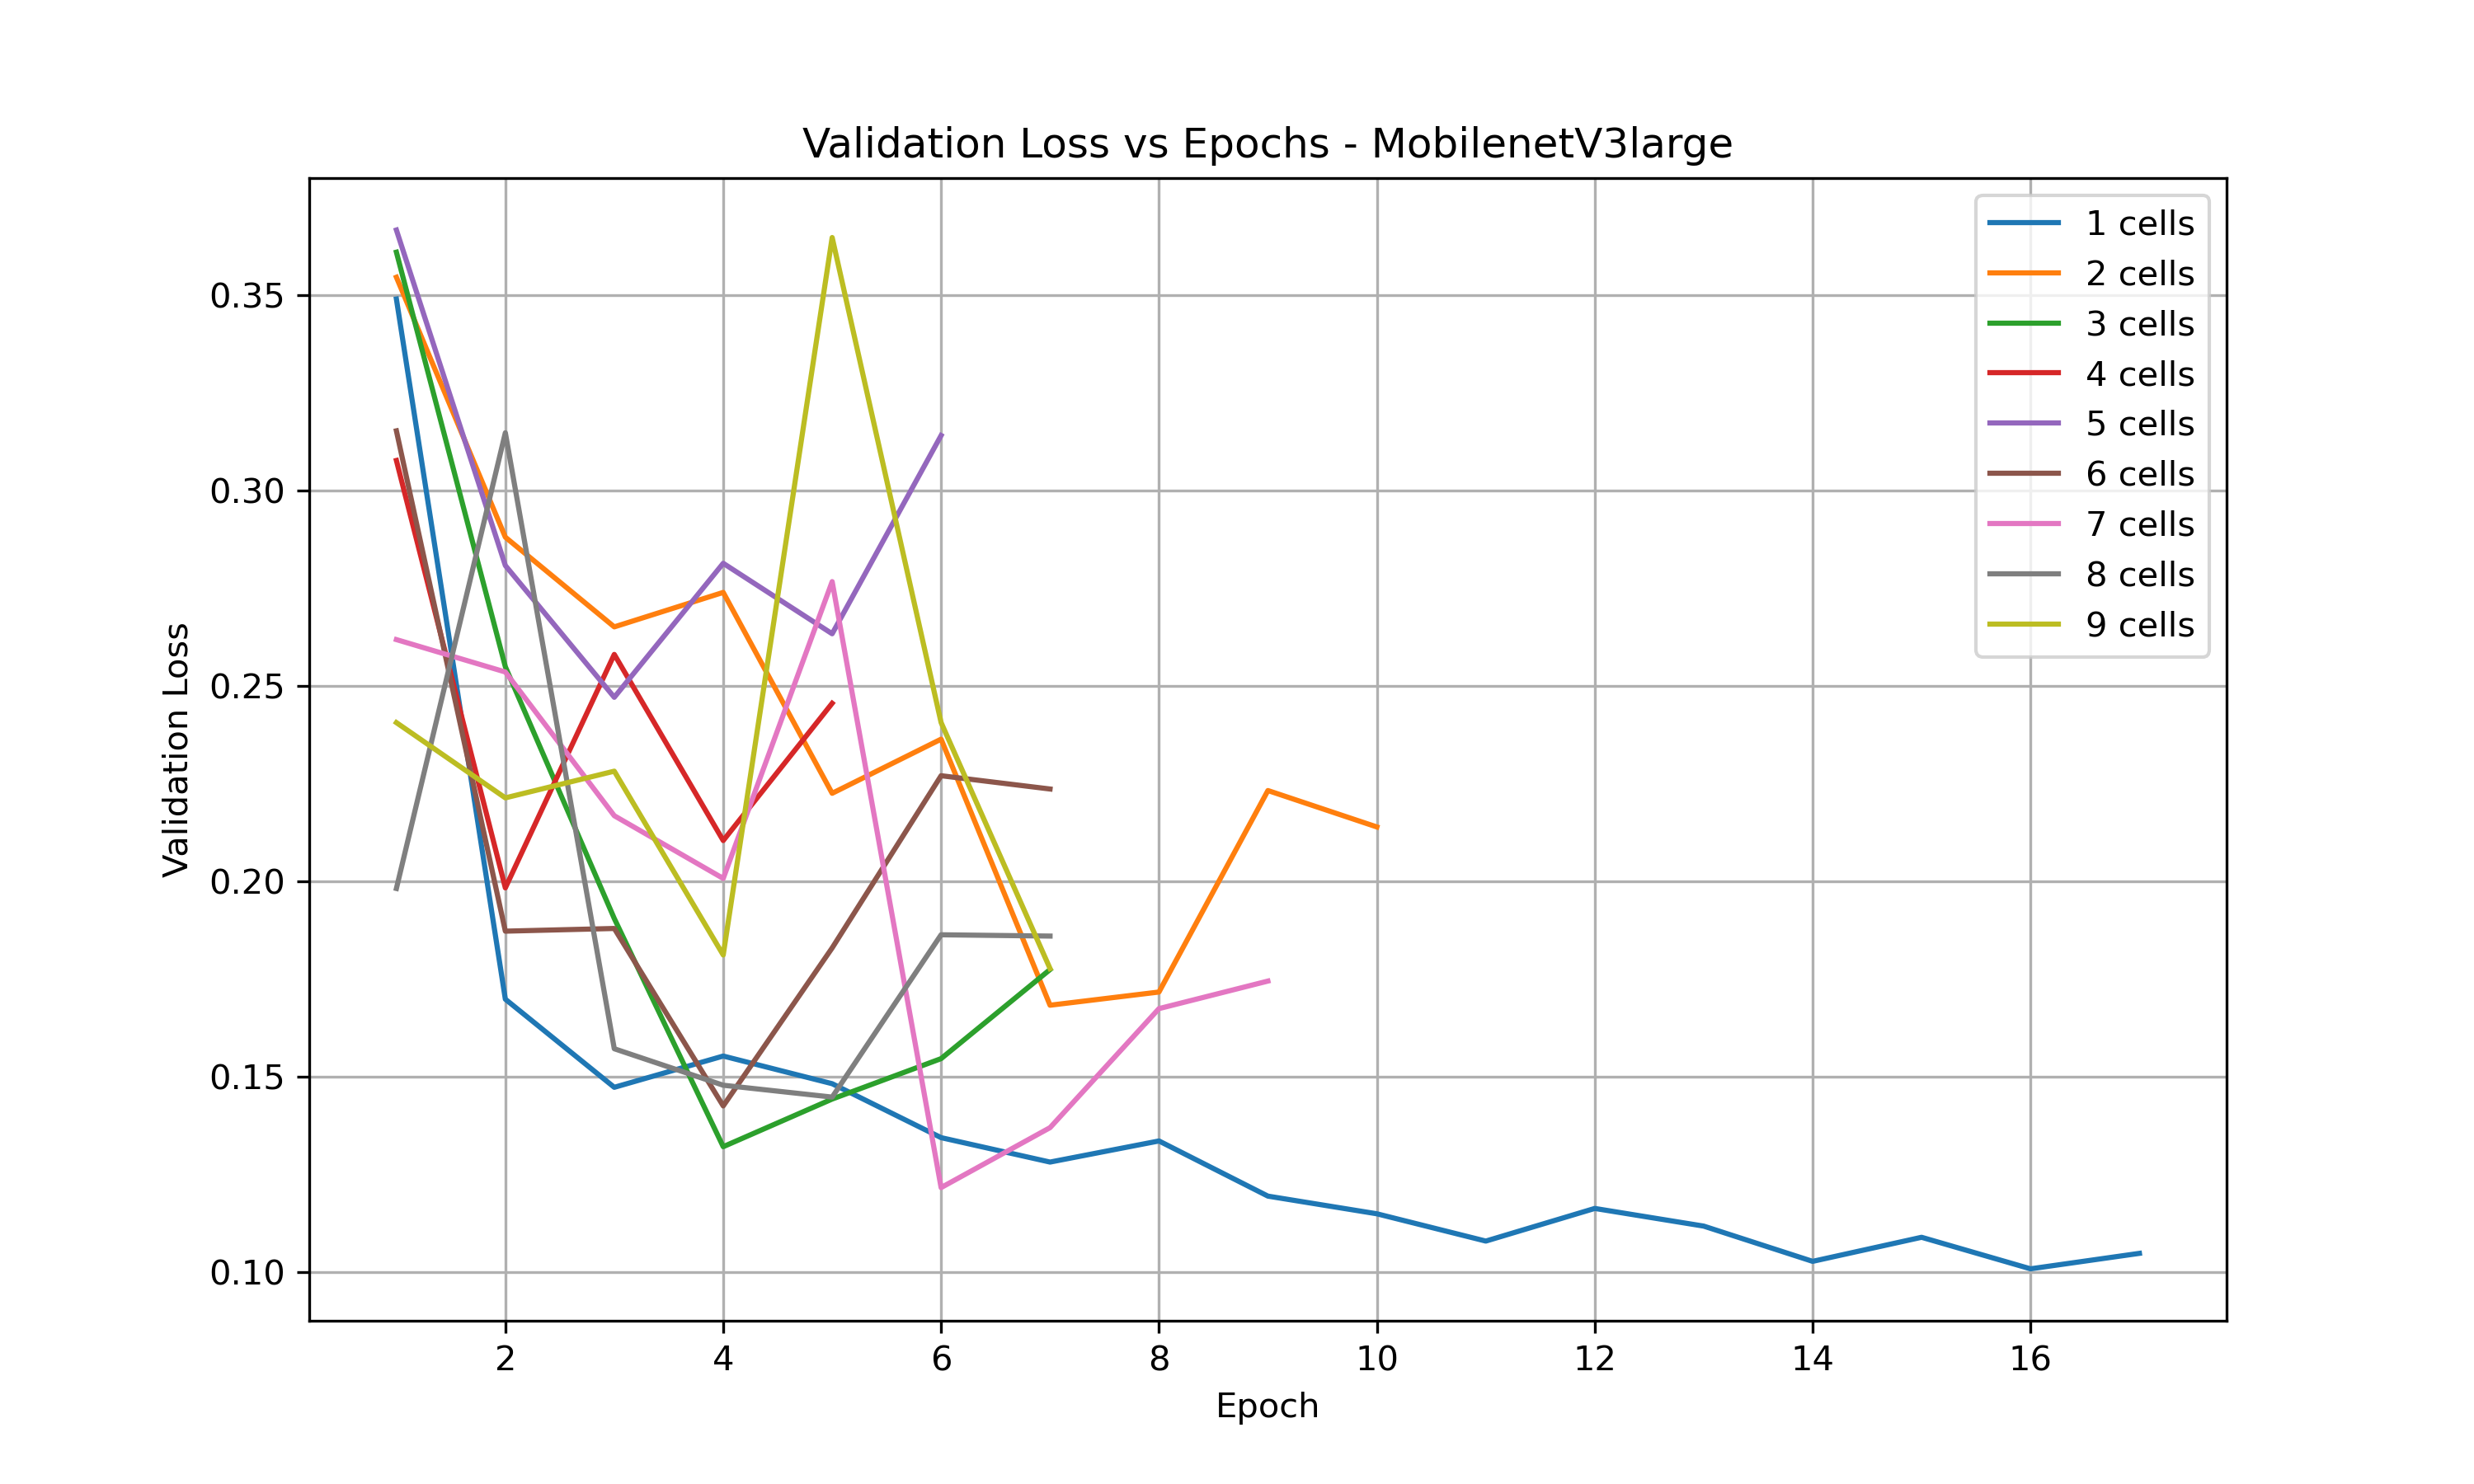
\includegraphics[width=0.48\textwidth]{../graphs/MobilenetV3large_val_loss_per_epoch.png}}
    \subfloat[\centering Pérdida por época]{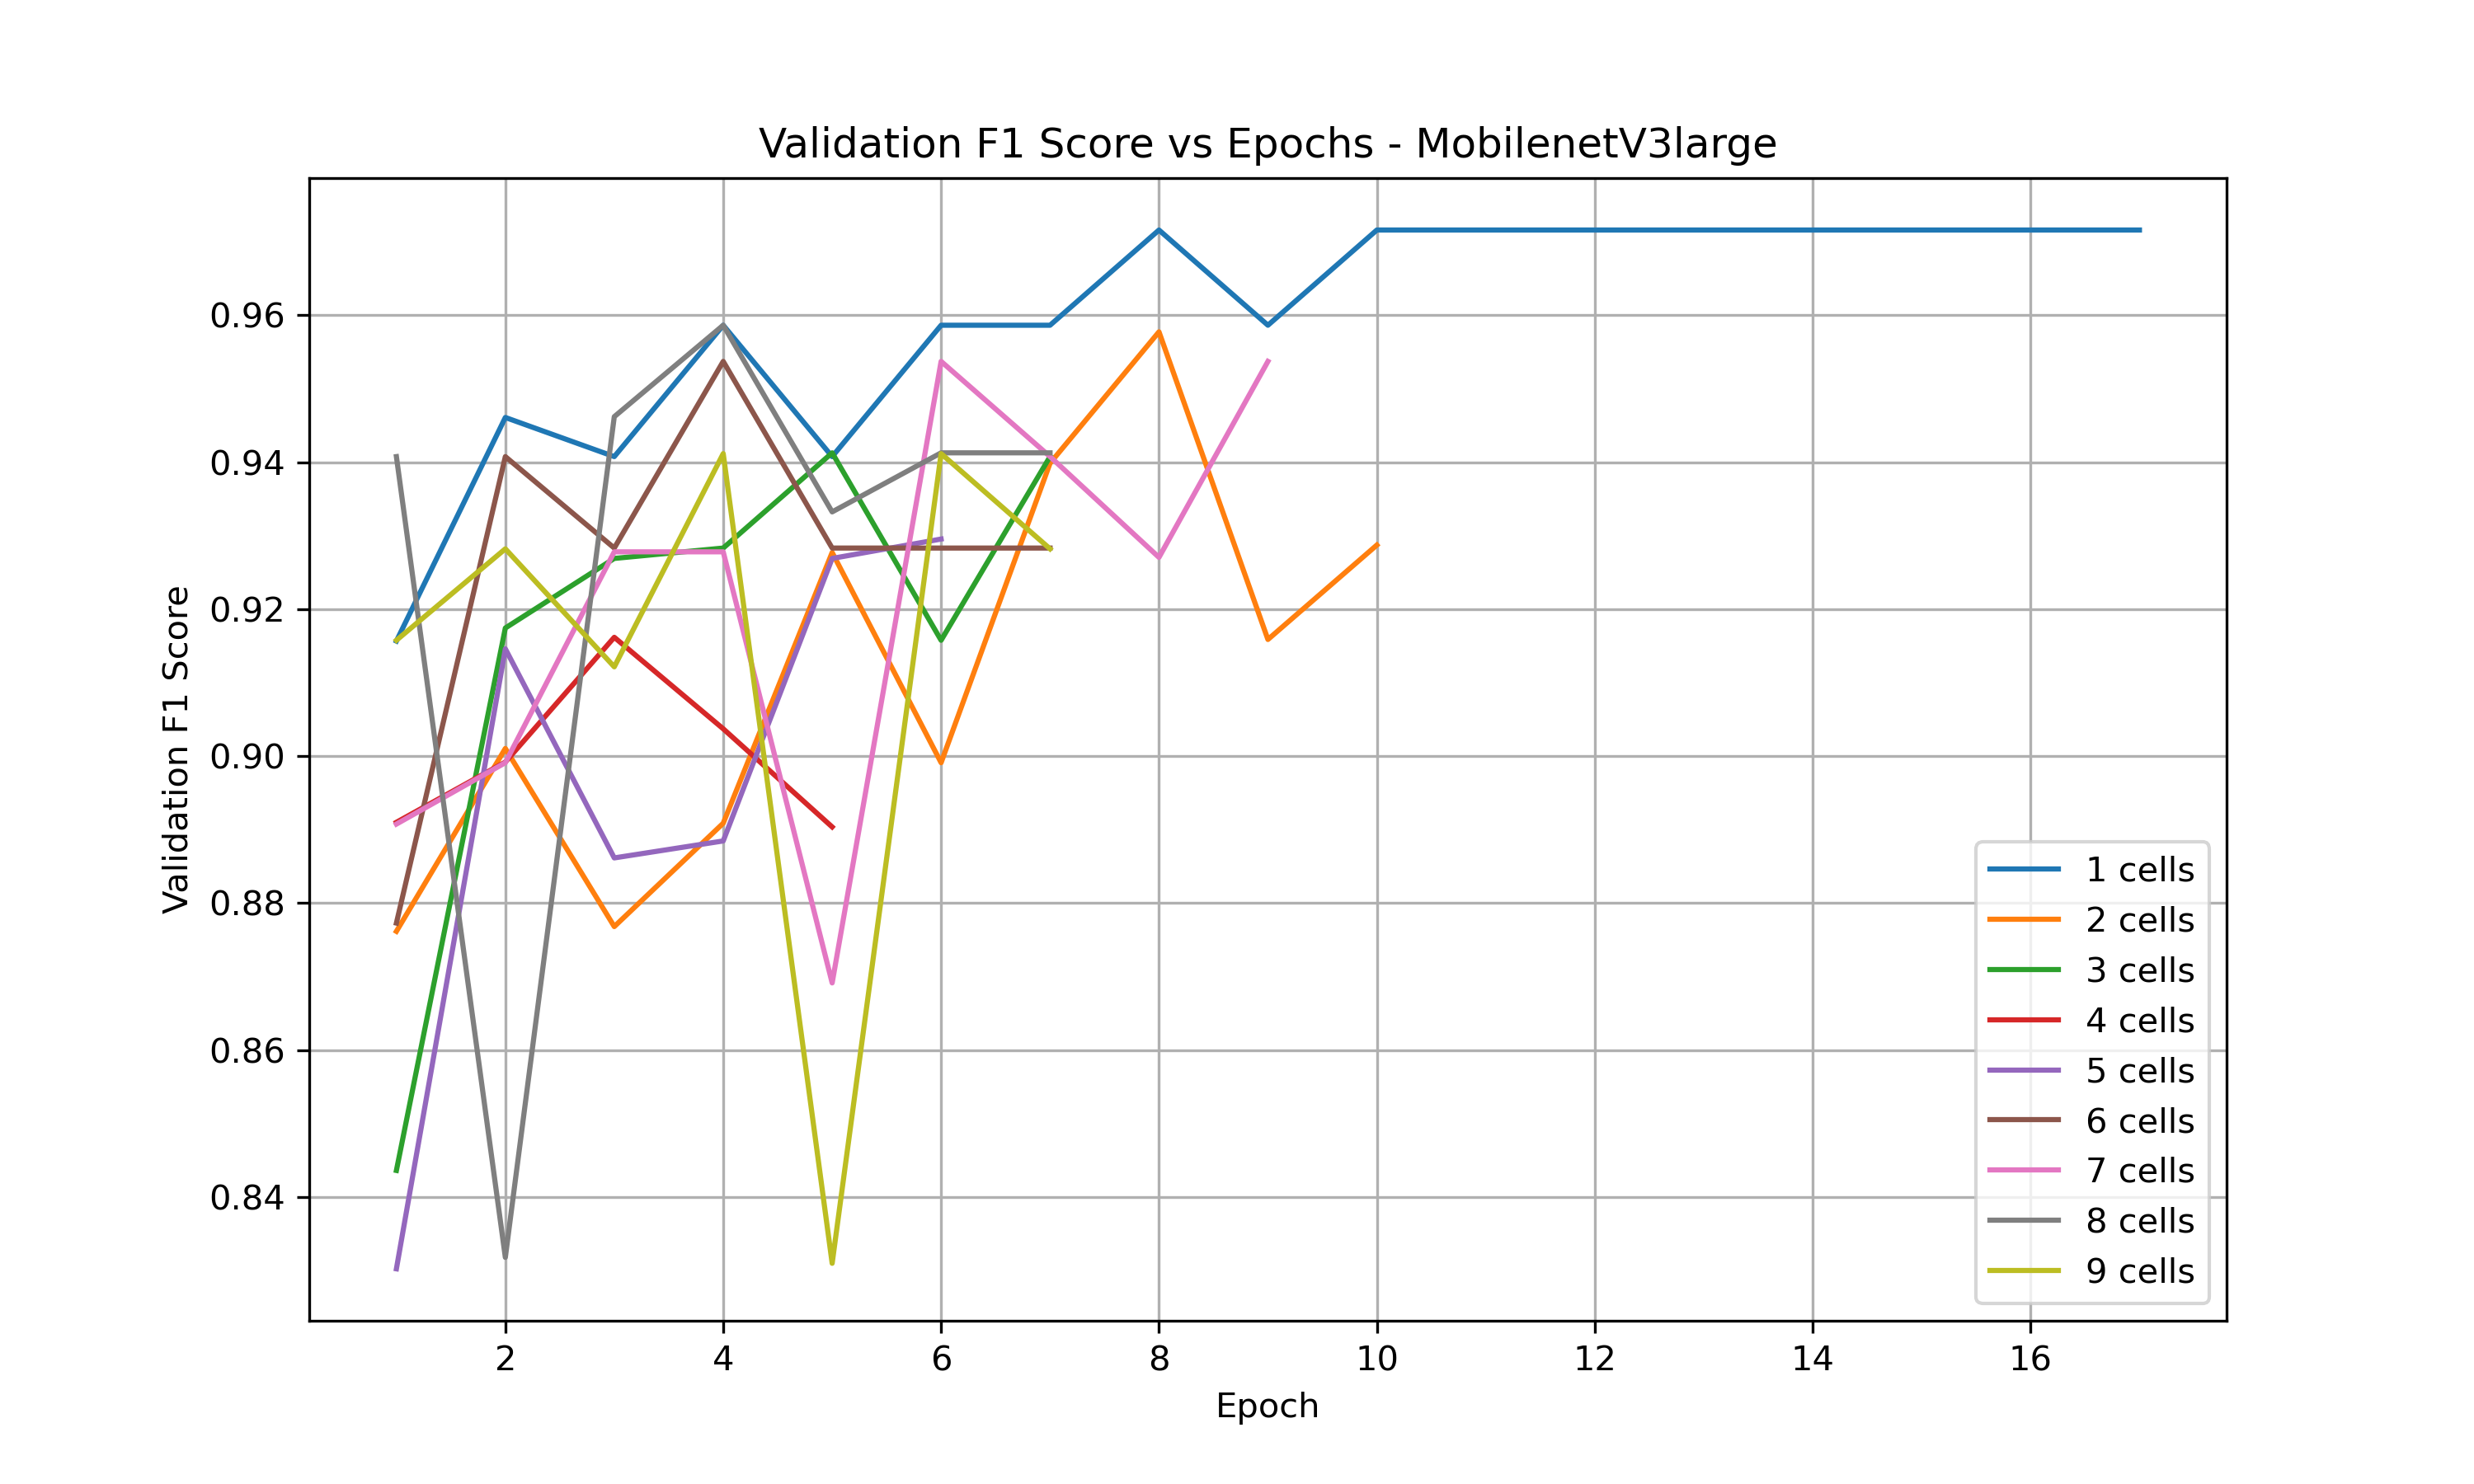
\includegraphics[width=0.48\textwidth]{../graphs/MobilenetV3large_val_f1_per_epoch.png}}\hfill
    \caption{Gráficos de pérdida y f1 score por época usando MobilenetV3}
    \label{fig:MobilenetV3}
\end{figure}

Utilizando MobileNetV3 se obtuvo un patrón muy distintivo entre la 
gráfica de pérdida y f1 score. En ambos casos se tuvo un descenso de 
pérdida muy estables utilizando la configuración de una sola celda, 
mientras que las demás se comportaron muy erráticamente. Esto es 
probablemente debido a la configuración del modelo, ya que es uno de 
los más ligeros del estado del arte (y también de entre los utilizados 
para esta experimentación). En ese sentido, las configuraciones con 
múltiples celdas cayeron en un overfitting para los vectores de 
características salidos de la CNN, por ende generando valores negativos 
en ambas métricas. 

\begin{figure}[h!]
    \centering
    \subfloat[\centering F1 score por época]{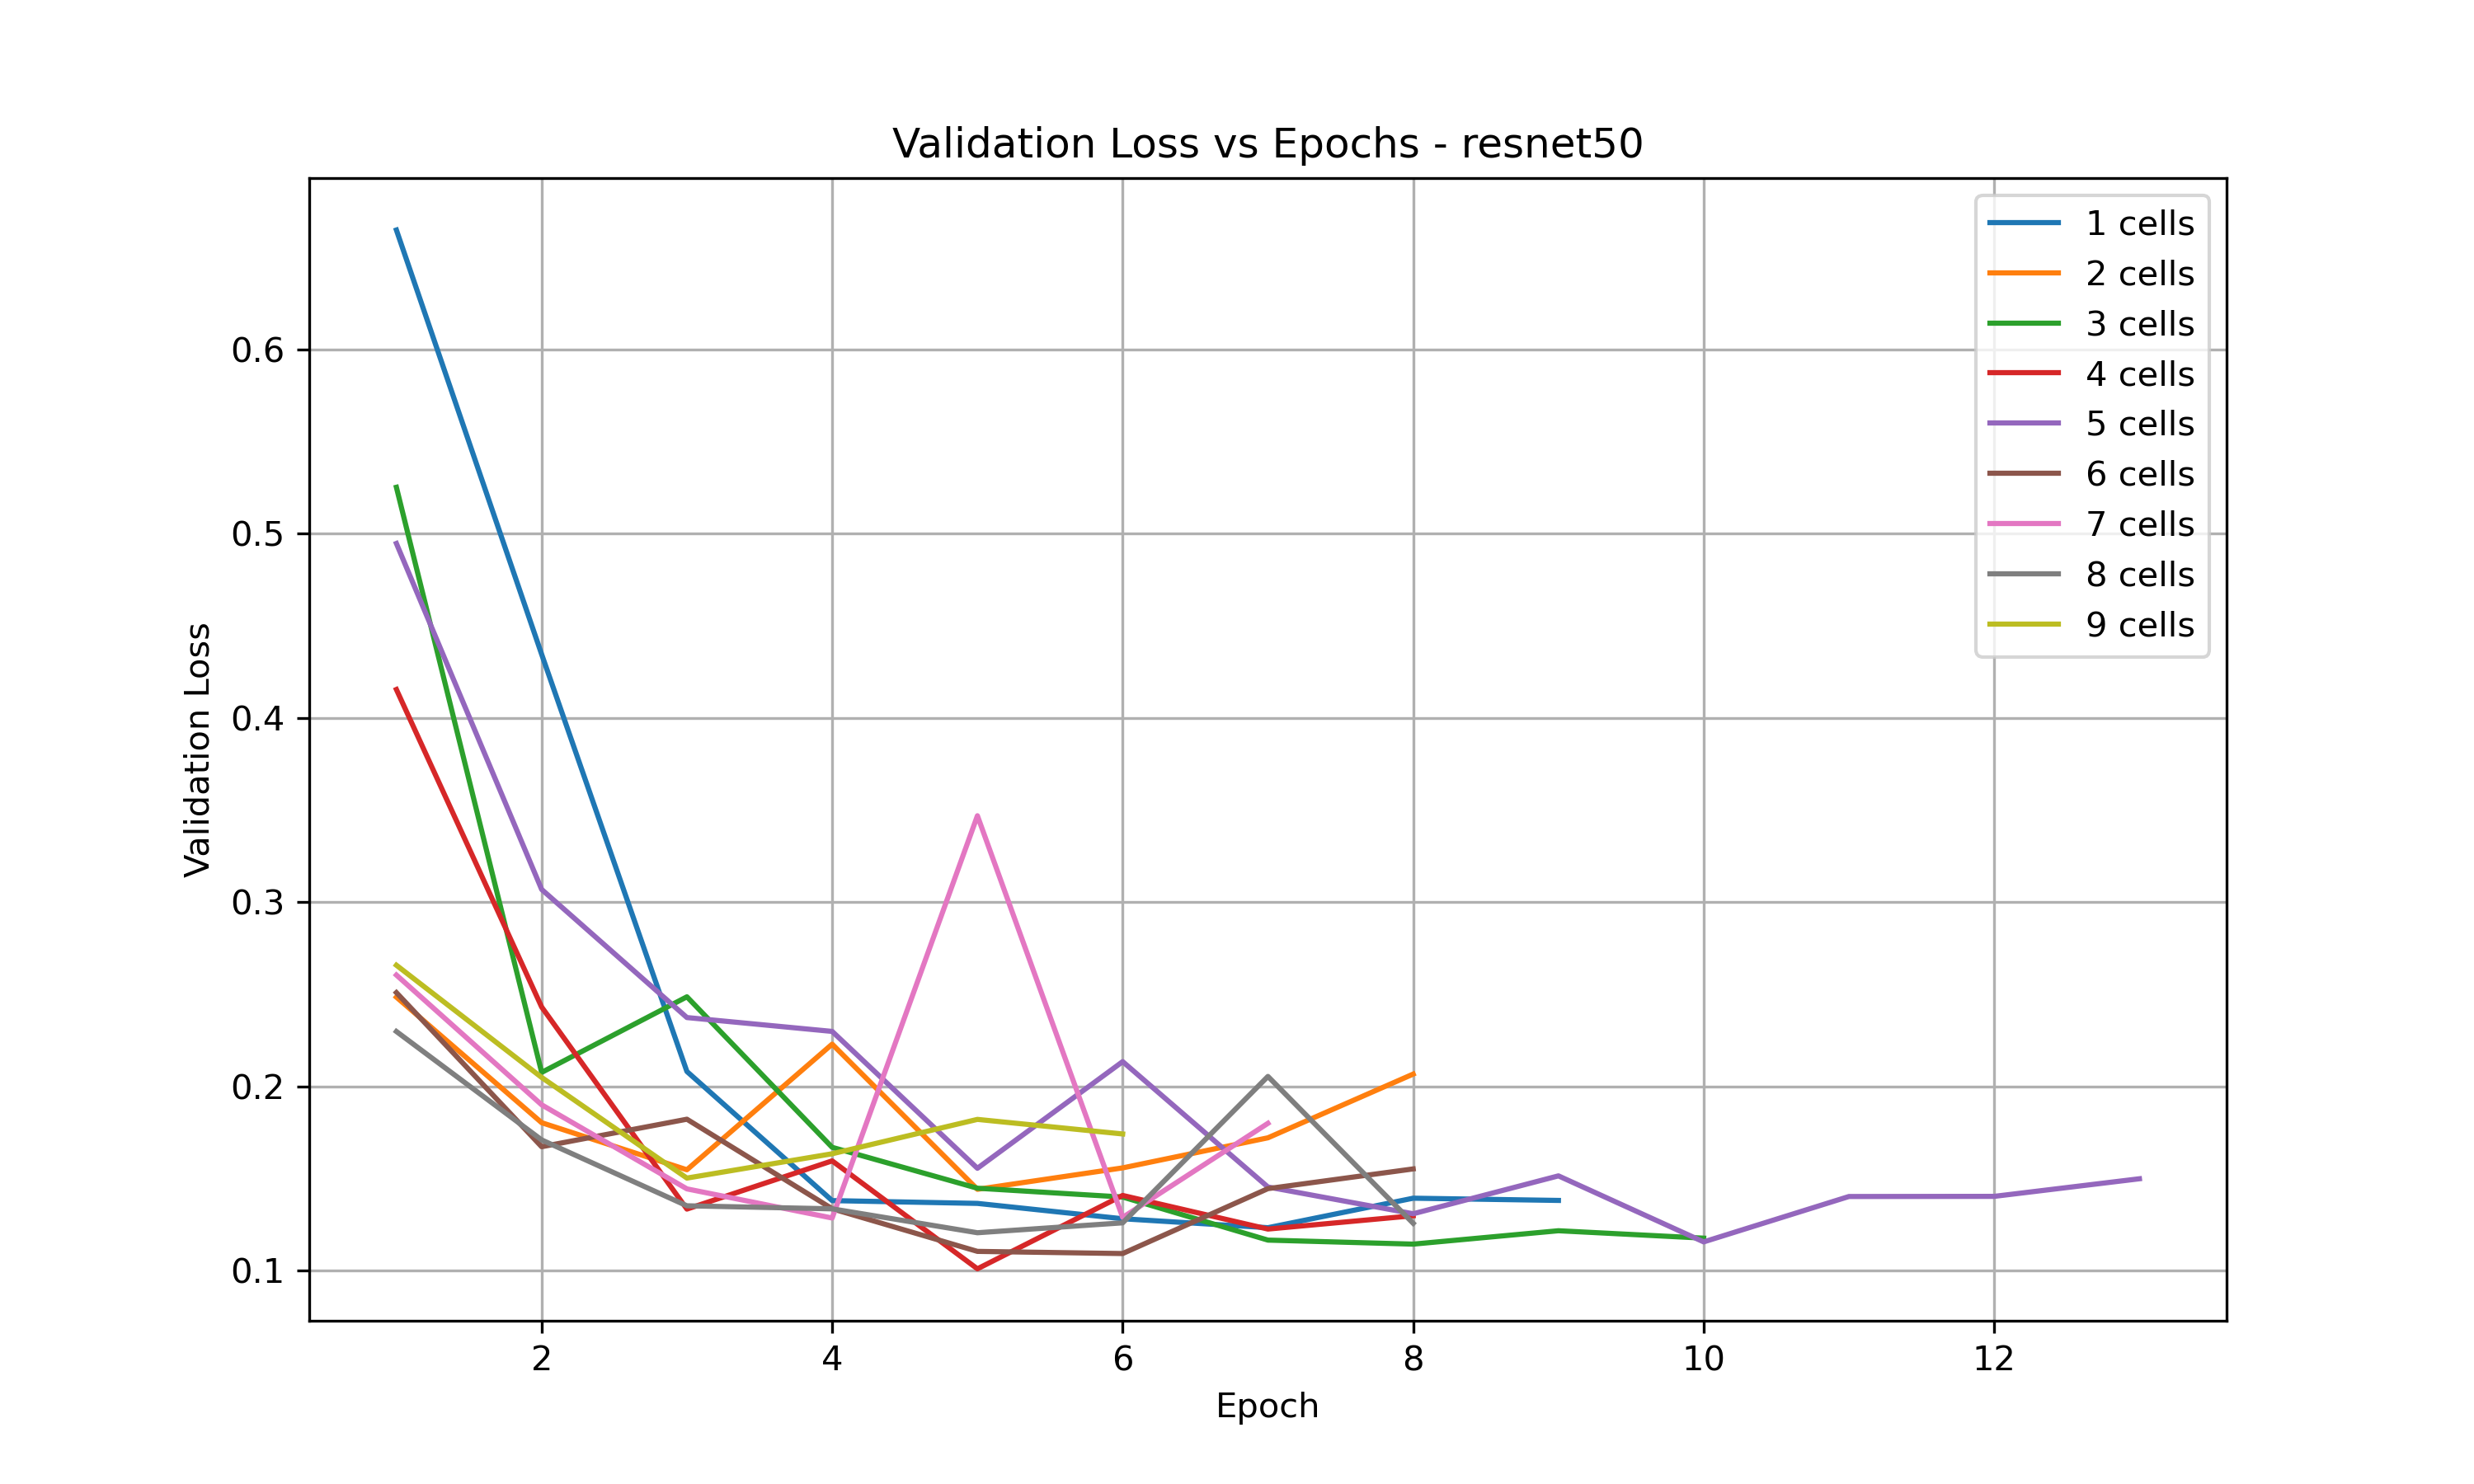
\includegraphics[width=0.48\textwidth]{../graphs/resnet50_val_loss_per_epoch.png}}
    \subfloat[\centering Pérdida por época]{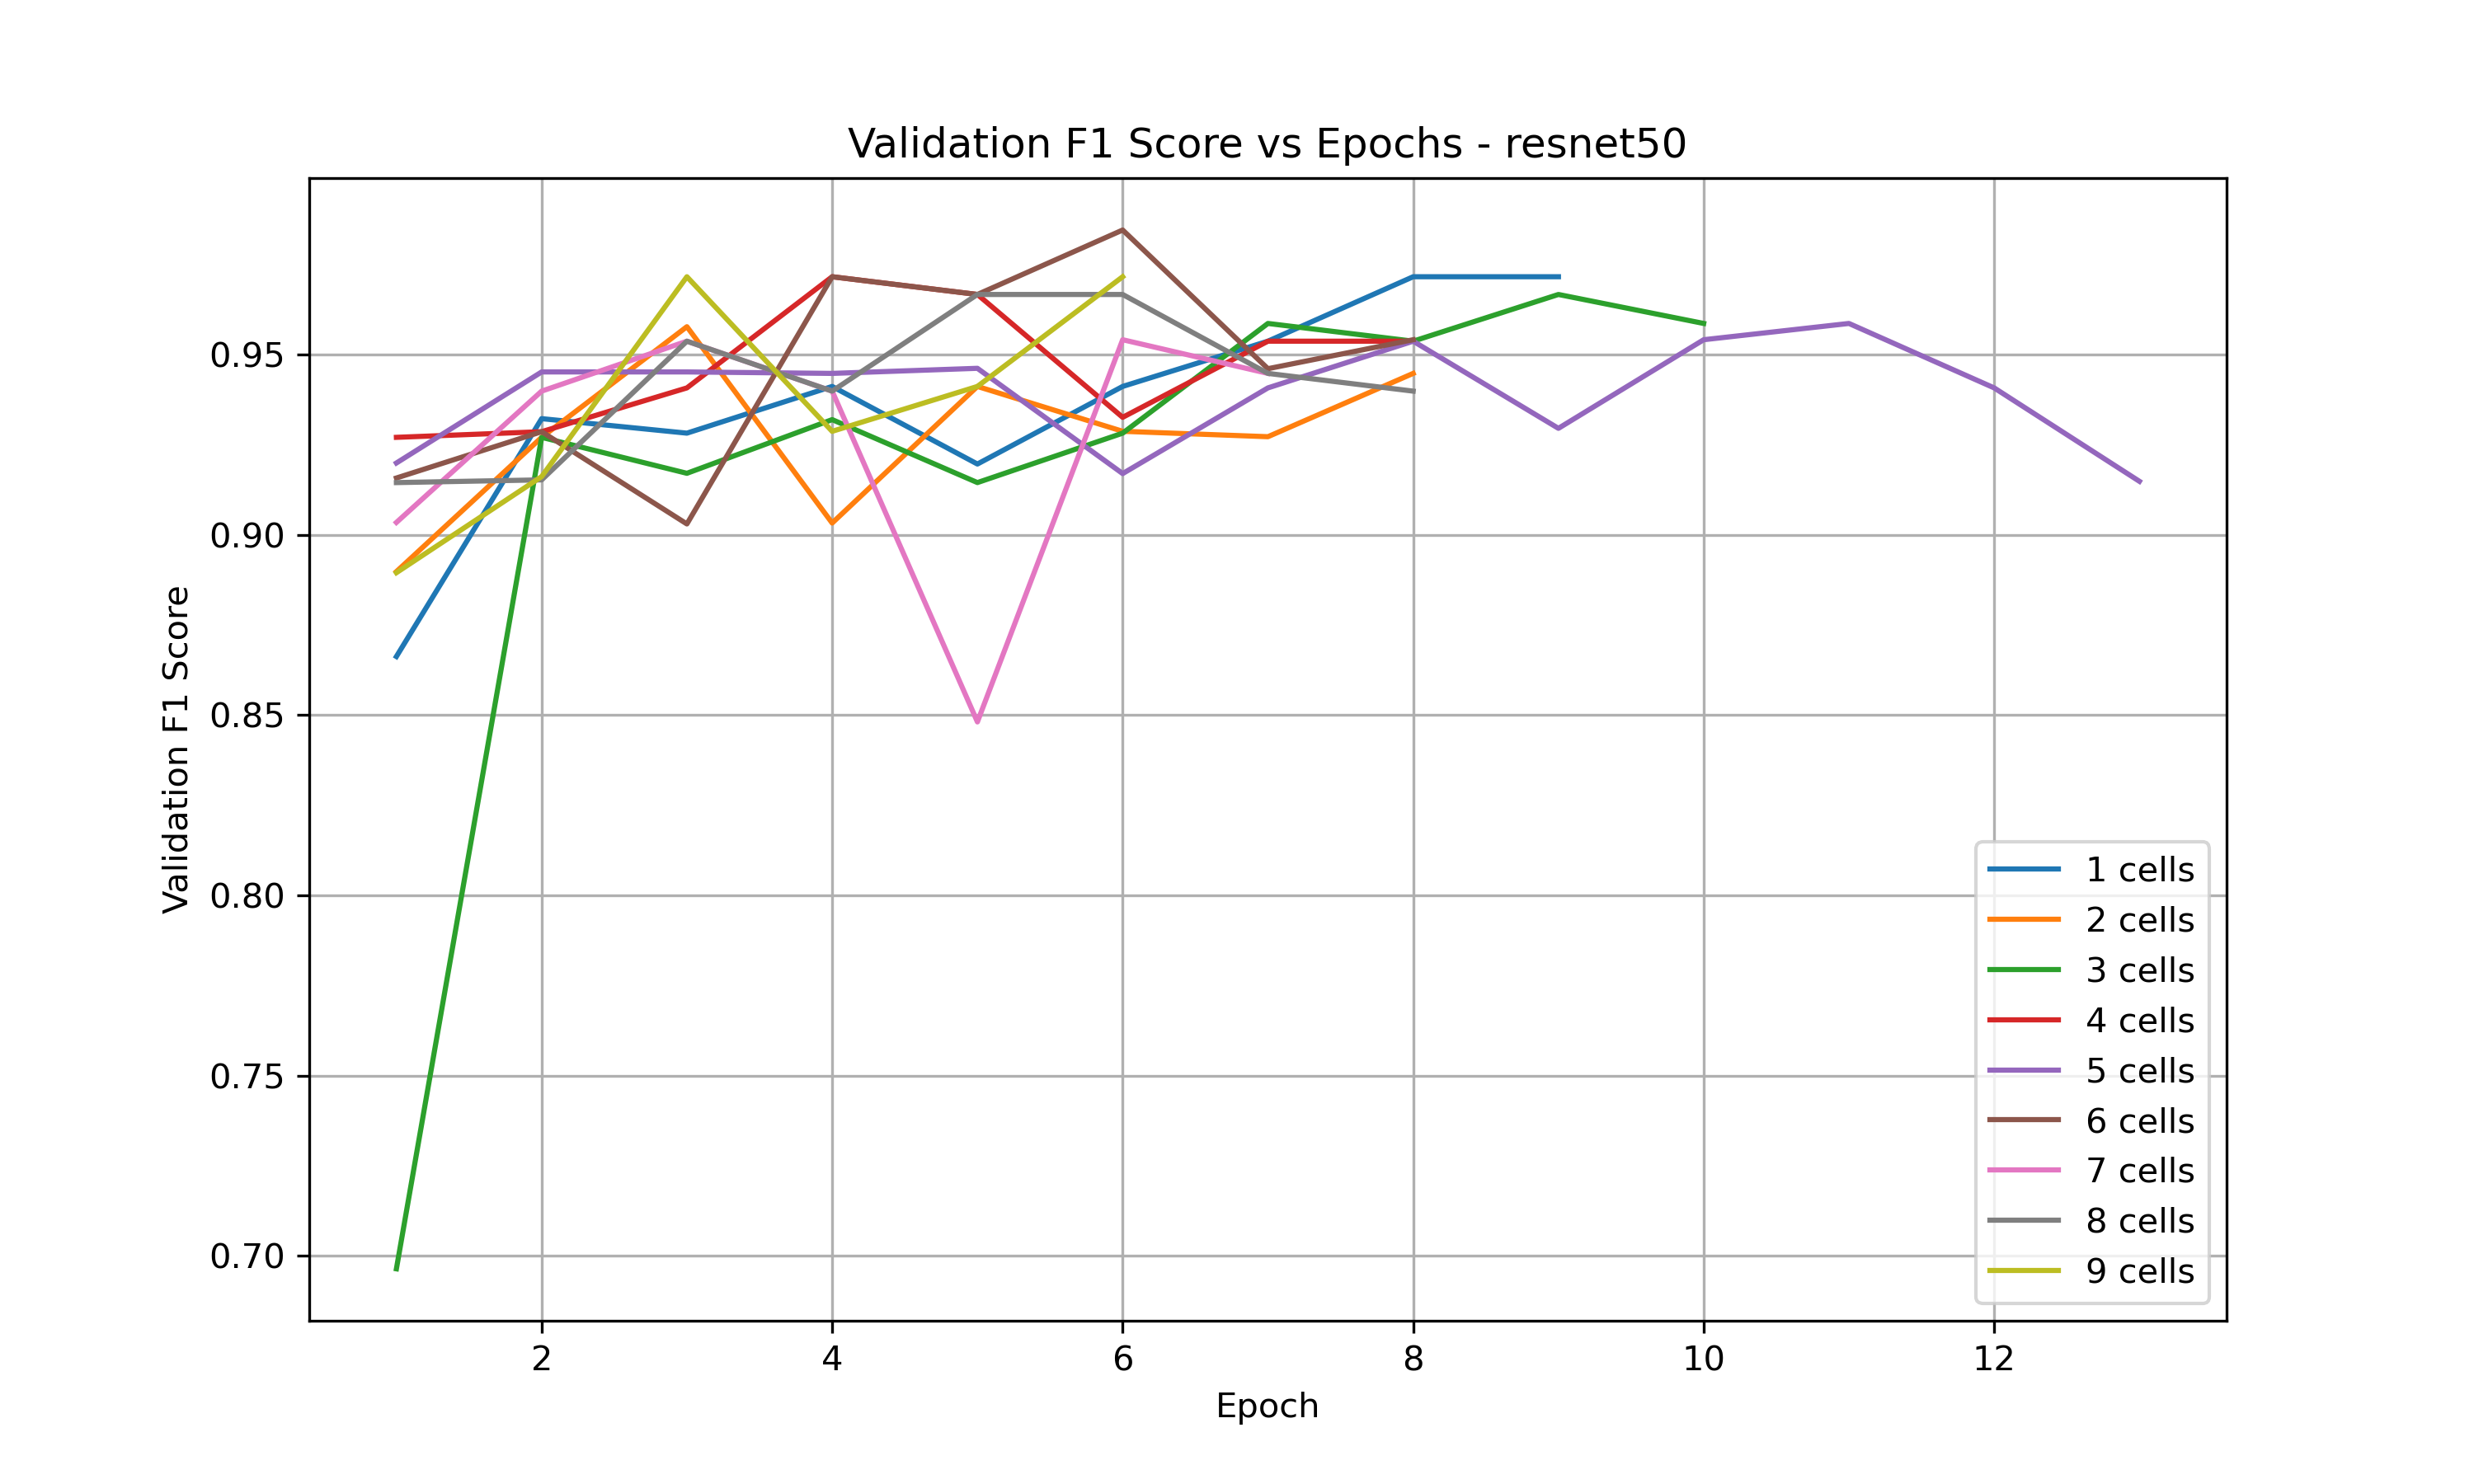
\includegraphics[width=0.48\textwidth]{../graphs/resnet50_val_f1_per_epoch.png}}\hfill
    \caption{Gráficos de pérdida y f1 score por época usando Resnet50}
    \label{fig:Resnet50}
\end{figure}

Las ejecuciones de Resnet50 generaron patrones más estables 
en ambos gráficos. En ese sentido la mayoría tuvo un descenso 
de la pérdida bastante similar entre ellos. Al compararlos 
teniendo en cuenta el early stopping, en la época 6 se 
generó una menor pérdida con el modelo de 6 épocas, lo cuál 
también concordó con ser el modelo con mejor f1 score de entre 
todos. Un dato interesante a analizar es el de la configuración 
con 7 celdas, el cual generó picos erráticos en el entrenamiento, 
lo cual también se reflejó en el gráfico de f1 score. Además, 
la configuración de 5 celdas tuvo una mayor cántidad de épocas 
de entrenamiento a comparación de los demás.

A continuación se muestran las métricas finales por cada uno de 
los modelos:

\begin{table}[h!]
\centering
\begin{tabular}{|l|l|l|l|l|l|l|}
\hline
\textbf{lstm\_cells} & \textbf{train\_loss} & \textbf{train\_f1} & \textbf{val\_loss} & \textbf{val\_f1} & \textbf{test\_loss} & \textbf{test\_f1} \\ \hline
\textbf{1}           & 0.0347               & 0.9873             & 0.2488             & 0.9408           & 0.0974              & 0.9725            \\ \hline
\textbf{2}           & 0.1213               & 0.9564             & 0.2392             & 0.9399           & 0.1674              & 0.9525            \\ \hline
\textbf{3}           & 0.0209               & 0.9902             & 0.1862             & 0.958            & 0.0698              & 0.9825            \\ \hline
\textbf{4}           & 0.047                & 0.9929             & \textbf{0.1038}    & 0.9541           & 0.1133              & 0.9575            \\ \hline
\textbf{5}           & 0.058                & 0.979              & 0.1506             & 0.9581           & 0.1049              & 0.97              \\ \hline
\textbf{6}           & 0.029                & 0.9931             & 0.1599             & 0.9541           & 0.0919              & 0.9725            \\ \hline
\textbf{7}           & 0.0258               & 0.9933             & 0.1367             & 0.9541           & 0.0691              & \textbf{0.985}    \\ \hline
\textbf{8}           & 0.0214               & 0.9929             & 0.2205             & 0.9412           & 0.1213              & 0.9625            \\ \hline
\textbf{9}           & \textbf{0.012}       & \textbf{0.9961}    & 0.1564             & \textbf{0.9667}  & \textbf{0.0605}     & \textbf{0.98}     \\ \hline
\end{tabular}
\caption{ Tabla comparativa de las métricas obtenidas por configuración de celdas para EfficientNetB0.}
\label{table:efficientnetb0Metrics}
\end{table}


En la tabla \ref{table:efficientnetb0Metrics} se las tienen 
métricas de pérdida y f1 score para todas las etapas: 
entrenamiento, validación y testeo para cada una de las 
configuraciones. En ella se puede ver que los mejores 
resultados de manera casi general fue la configuración de 9 
celdas, lo cual no se refleja con los resultados de validación 
que se vieron en los gráficos de pérdida y f1 score anteriormente 
mostrados. 


\begin{table}[h!]
\centering
\begin{tabular}{|l|l|l|l|l|l|l|}
\hline
\textbf{lstm\_cells} & \textbf{train\_loss} & \textbf{train\_f1} & \textbf{val\_loss} & \textbf{val\_f1} & \textbf{test\_loss} & \textbf{test\_f1} \\ \hline
\textbf{1}  & 0.0833               & 0.9693             & 0.2338             & 0.932            & 0.12                & 0.9675            \\ \hline
\textbf{2}  & 0.048                & 0.9869             & \textbf{0.1492}    & \textbf{0.9586}  & 0.0849              & 0.9775            \\ \hline
\textbf{3}  & 0.185                & 0.9349             & 0.3138             & 0.8779           & 0.2181              & 0.9175            \\ \hline
\textbf{4}  & 0.1111               & 0.9605             & 0.268              & 0.9187           & 0.1375              & 0.96              \\ \hline
\textbf{5}  & 0.0228               & 0.9936             & 0.1915             & 0.927            & 0.0666              & \textbf{0.9825}   \\ \hline
\textbf{6}  & 0.0396               & 0.9875             & 0.1626             & \textbf{0.9537}  & 0.0789              & \textbf{0.98}     \\ \hline
\textbf{7}  & 0.1473               & 0.9402             & 0.2269             & 0.932            & 0.1458              & 0.96              \\ \hline
\textbf{8}  & 0.0504               & 0.9872             & 0.1829             & 0.9139           & 0.1408              & 0.95              \\ \hline
\textbf{9}  & \textbf{0.018}       & \textbf{0.9969}    & 0.2741             & 0.9295           & \textbf{0.0649}     & \textbf{0.9825}   \\ \hline
\end{tabular}
\caption{ Tabla comparativa de las métricas obtenidas por configuración de celdas para EfficientnetV2.}
\label{table:efficientnetV2Metrics}
\end{table}

A comparación de la anterior tabla, utilizando los datos de la tabla 
\ref{table:efficientnetV2Metrics} no se puede sacar una conclusión 
específica acerca de cual configuración es la mejor a comparación del resto. 
Esto se puede ver debido a que los mejores resultados (obtenidos con 9 celdas) 
son diferentes para validación que para entrenamiento y testing. Además, 
al revisar los datos de los gráficos de validación mostrados anteriormente, se 
pudo ver que este estaba generando un ligero overfitting. 

\begin{table}[h!]
\centering
\begin{tabular}{|l|l|l|l|l|l|l|}
\hline
\textbf{lstm\_cells} & \textbf{train\_loss} & \textbf{train\_f1} & \textbf{val\_loss} & \textbf{val\_f1} & \textbf{test\_loss} & \textbf{test\_f1} \\ \hline
\textbf{1}           & 0.0562               & 0.9875             & \textbf{0.1048}    & \textbf{0.9716}  & \textbf{0.0721}     & \textbf{0.9825}   \\ \hline
\textbf{2}           & 0.0527               & 0.9845             & 0.2139             & 0.9287           & 0.1006              & 0.9775            \\ \hline
\textbf{3}           & \textbf{0.0237}      & \textbf{0.9969}    & 0.1774             & 0.9408           & 0.1117              & 0.965             \\ \hline
\textbf{4}           & 0.092                & 0.9655             & 0.2456             & 0.8904           & 0.1914              & 0.935             \\ \hline
\textbf{5}           & 0.1141               & 0.9649             & 0.3142             & 0.9295           & 0.1982              & 0.9325            \\ \hline
\textbf{6}           & 0.0376               & 0.987              & 0.2237             & 0.9283           & 0.1158              & 0.97              \\ \hline
\textbf{7}           & 0.0376               & 0.986              & 0.1745             & 0.9537           & \textbf{0.0706}     & 0.9775            \\ \hline
\textbf{8}           & 0.0497               & 0.986              & 0.186              & 0.9413           & 0.1219              & 0.965             \\ \hline
\textbf{9}           & 0.0807               & 0.9772             & 0.1777             & 0.9282           & 0.1368              & 0.9625            \\ \hline
\end{tabular}
\caption{ Tabla comparativa de las métricas obtenidas por configuración de celdas para MobileNetV3.}
\label{table:MobileNetV3Metrics}
\end{table}

La tabla \ref{table:MobileNetV3Metrics} muestra resultados más 
concluyentes a comparación de las demás. Al igual que con los gráficos 
anteriores, se puede ver que si bien no se obtuvieron los mejores 
resultados finales para entrenamiento, si lo hizo para prueba y testeo. 
Además, se puede ver que estos empeoran mientras más celdas de BI-LSTM 
se usan. En ese sentido, se puede afirmar que esta es la mejor 
configuración para este modelo, 

\begin{table}[h!]
\centering
\begin{tabular}{|l|l|l|l|l|l|l|}
\hline
\textbf{lstm\_cells} & \textbf{train\_loss} & \textbf{train\_f1} & \textbf{val\_loss} & \textbf{val\_f1} & \textbf{test\_loss} & \textbf{test\_f1} \\ \hline
\textbf{1}           & 0.1039               & 0.9769             & 0.1382             & \textbf{0.9716}  & 0.116               & 0.9725            \\ \hline
\textbf{2}           & 0.0907               & 0.9808             & 0.2067             & 0.9448           & 0.1111              & 0.97              \\ \hline
\textbf{3}           & 0.0837               & 0.9771             & \textbf{0.1177}    & 0.9586           & 0.1183              & 0.9675            \\ \hline
\textbf{4}           & \textbf{0.0471}      & \textbf{0.9904}    & 0.1298             & 0.9537           & \textbf{0.0858}     & \textbf{0.98}     \\ \hline
\textbf{5}           & \textbf{0.049}       & \textbf{0.993}     & 0.1499             & 0.9148           & \textbf{0.0866}     & \textbf{0.9775}   \\ \hline
\textbf{6}           & 0.0925               & 0.9649             & 0.1553             & 0.9541           & 0.0973              & 0.975             \\ \hline
\textbf{7}           & 0.1106               & 0.9551             & 0.18               & 0.9448           & 0.1374              & 0.9525            \\ \hline
\textbf{8}           & 0.1262               & 0.9576             & 0.1257             & 0.9399           & 0.1074              & 0.975             \\ \hline
\textbf{9}           & 0.0624               & 0.9872             & 0.1742             & \textbf{0.9716}  & 0.1188              & 0.97              \\ \hline
\end{tabular}
\caption{ Tabla comparativa de las métricas obtenidas por configuración de celdas para Resnet50.}
\label{table:Resnet50}
\end{table}

Observando los datos de la tabla \ref{table:Resnet50} es 
notorio que los mejores resultados estuvieron en las 
configuraciones medias (4 y 5 celdas). Además también se 
logra idntificar que mientras más o menos celdas, todas las 
métricas se reducen, salvo con el caso de 9 celdas, el cual 
es un dato anómalo en esa distribución. 

Por último, a continuación se mostrará una tabla comparativa 
resumen de toda la experimentación realizada en el presente trabajo: 

\begin{table}[h!]
\centering
\begin{tabular}{|l|l|l|l|l|l|l|l|}
\hline
\textbf{cnn\_model}     & \textbf{lstm\_cells} & \textbf{train\_loss} & \textbf{train\_f1} & \textbf{val\_loss} & \textbf{val\_f1} & \textbf{test\_loss} & \textbf{test\_f1} \\ \hline
\textbf{EfficientNetB0} & 9                    & \textbf{0.012}       & \textbf{0.9961}    & 0.1564             & \textbf{0.9716}  & \textbf{0.0605}     & \textbf{0.98}     \\ \hline
\textbf{EfficientNetV2} & 9                    & 0.018                & \textbf{0.9969}    & 0.2741             & 0.9295           & \textbf{0.0649}     & \textbf{0.9825}   \\ \hline
\textbf{MobileNetV3}    & 1                    & 0.0562               & 0.9875             & \textbf{0.1048}    & \textbf{0.9716}  & 0.0721              & \textbf{0.9825}   \\ \hline
\textbf{ResNet50}       & 4                    & 0.0471               & 0.9904             & 0.1298             & 0.9537           & 0.0858              & \textbf{0.98}     \\ \hline
\end{tabular}
\caption{ Tabla comparativa resumen final de la experimentación}
\label{table:Resnet50}
\end{table}

Con los resultados finales se puede corroborar que todas las 
combinaciones entre CNN y LSTM lograron valores similares para 
todas las métricas de testeo al tener un f1 score . En ese sentido, 
y con el fin de optimizar el \textit{pipeline} final para el 
\textit{dataset} propuesto, sería recomendable utilizar MobileNetV3 
con una celda LSTM, ya que proporcionó el mismo resultado pero tanto 
el peso del modelo como el número de celdas es menor que en todas las 
demás configuraciones.
